\documentclass[a4paper]{article}

% CJK support: prefer ctex, fallback to XeTeX native line breaking
\IfFileExists{ctex.sty}{
  \usepackage[fontset=fandol]{ctex}
}{
  % Fallback for minimal TeX installs (e.g. MacTeX Basic, TeX Live scheme-basic)
  % without ctex/xeCJK. Uses XeTeX's built-in CJK line breaking.
  \usepackage{fontspec}
  \XeTeXlinebreaklocale "zh"
  \XeTeXlinebreakskip = 0pt plus 1pt
  \IfFontExistsTF{Songti SC}{\setmainfont{Songti SC}}{%
    \IfFontExistsTF{Noto Serif CJK SC}{\setmainfont{Noto Serif CJK SC}}{}%
  }
  \IfFontExistsTF{Heiti SC}{\setsansfont{Heiti SC}}{%
    \IfFontExistsTF{Noto Sans CJK SC}{\setsansfont{Noto Sans CJK SC}}{}%
  }
}

% Basic packages
\usepackage{amsmath, amssymb}
\usepackage{graphicx}
\usepackage[margin=2.5cm]{geometry}
\emergencystretch=3em
\usepackage[most]{tcolorbox}
\usepackage{etoolbox}
\usepackage{listings}
\usepackage{hyperref}
\usepackage{booktabs}
\usepackage{array}
\usepackage{subcaption}
\usepackage{float}
\usepackage{tikz}
\IfFileExists{pgfplots.sty}{
    \usepackage{pgfplots}
    \pgfplotsset{compat=1.18}
}{}

% ===== Highlight boxes =====
\newtcolorbox{knowledgebox}[1]{
    enhanced, colback=blue!5!white, colframe=blue!75!black, colbacktitle=blue!75!black,
    coltitle=white, fonttitle=\bfseries, title={#1}, attach boxed title to top left={yshift=-2mm, xshift=2mm},
    boxrule=1pt, sharp corners
}

\newtcolorbox{importantbox}[1]{
    enhanced, colback=yellow!10!white, colframe=yellow!80!black, colbacktitle=yellow!80!black,
    coltitle=black, fonttitle=\bfseries, title={#1}, sharp corners
}

\newtcolorbox{warningbox}[1]{
    enhanced, colback=red!5!white, colframe=red!75!black, colbacktitle=red!75!black,
    coltitle=white, fonttitle=\bfseries, title={#1}, sharp corners
}

\newtcolorbox{practicebox}[1]{
    enhanced, colback=black!3!white, colframe=black!75, colbacktitle=black!75,
    coltitle=white, fonttitle=\bfseries, title={#1}, sharp corners
}

% ===== Code listings =====
\lstset{
    basicstyle=\ttfamily\small,
    keywordstyle=\color{blue},
    stringstyle=\color{red!60!black},
    commentstyle=\color{green!60!black},
    breaklines=true,
    frame=single,
    numbers=left,
    numberstyle=\tiny\color{gray},
    captionpos=b,
    extendedchars=false
}

% ===== Figure provenance and unit macros =====
% \vtag goes inside \caption{...}; \srcnote{MM:SS--MM:SS} follows the figure environment.
\newcommand{\vtag}{\protect\footnotemark}
\newcommand{\srcnote}[1]{\footnotetext{视频画面时间区间：#1。若为裁剪图，时间区间仍对应原视频画面。}}
% Units work in text and math mode; never hand-write $^\circ$ or \AA inside \mathrm.
\newcommand{\degC}{\ensuremath{^{\circ}\mathrm{C}}}
\newcommand{\um}{\ensuremath{\mu\mathrm{m}}}
\newcommand{\nm}{\ensuremath{\mathrm{nm}}}
\newcommand{\angstrom}{\ensuremath{\text{\AA}}}

% ===== Front-page metadata =====
% Fill these in when generating notes.
\newcommand{\notetitle}{奇异值分解与主成分分析}
\newcommand{\notesubtitle}{GAMES001 图形学中的数学 · 第 5 集：实对称矩阵、SVD、伪逆、极分解、形状匹配、图像压缩与 PCA}
\newcommand{\noteauthors}{根据 GAMES-Webinar 直播录像整理（阮良旺 主讲）}
\newcommand{\notedate}{2024年4月1日（直播）}
\newcommand{\videochannel}{GAMES-Webinar（哔哩哔哩）}
\newcommand{\videopublishdate}{2024年3月6日（合集）}
\newcommand{\videoduration}{1小时48分46秒}
\newcommand{\videourl}{https://www.bilibili.com/video/BV1MF4m1V7e3/?p=5}
\newcommand{\videocoverpath}{cover.jpg}

\begin{document}

% ===== Title page =====
\begin{titlepage}
\centering
{\Large 课程笔记\par}
\vspace{1.2cm}
{\huge\bfseries \notetitle\par}
\ifdefempty{\notesubtitle}{}{
\vspace{0.3cm}
{\large \notesubtitle\par}
}
\vspace{0.5cm}
{\large \noteauthors\par}
\vspace{0.3cm}
{\large \notedate\par}
\vspace{1.0cm}

\ifdefempty{\videocoverpath}{
{\small 请在生成笔记时填入视频封面图的本地路径。\par}
}{
\includegraphics[width=0.82\textwidth,height=0.40\textheight,keepaspectratio]{\videocoverpath}\par
}

\vfill
\begin{tcolorbox}[width=0.9\textwidth, colback=black!2!white, colframe=black!60, sharp corners]
\textbf{视频作者/频道}：\videochannel\par
\textbf{发布日期}：\videopublishdate\par
\textbf{视频时长}：\videoduration\par
\textbf{视频链接}：
\ifdefempty{\videourl}{
未填写
}{
\href{\videourl}{\nolinkurl{\videourl}}
}
\end{tcolorbox}
\end{titlepage}

\tableofcontents
\newpage

%% --- 正文内容开始 --- %%

\section{如何理解一个矩阵}

第五讲由阮良旺主讲，内容是奇异值分解（singular value decomposition, SVD）与主成分分析（principal component analysis, PCA）。直播当天是 4 月 1 日，讲者开场先祝大家愚人节快乐。

讲者从一个问题开始：如何理解一个矩阵？矩阵是一种非常通用的数据结构。它可以表达二维或三维的线性变换；可以单独表示一张图片，每个元素是一个像素；也可以表示一组几何数据，比如网格的顶点坐标排成的矩阵。把一片点云中每个点的坐标作为一行组合到一起，它也是一个矩阵。讲者提出的问题是：如何理解这些矩阵背后更深层次的含义，它们所表示的信息到底是什么？今天介绍的 SVD 就是回答这个问题的工具。无论矩阵代表什么，SVD 都能把它拆成“旋转—拉伸—旋转”三个结构清楚的部分，并按重要性排好序。前一张图展示了用 SVD 对一张图片做不同程度的低秩近似，保留的分量越多，图像越清晰。

\noindent\begin{minipage}{\textwidth}
\begin{figure}[H]
\centering
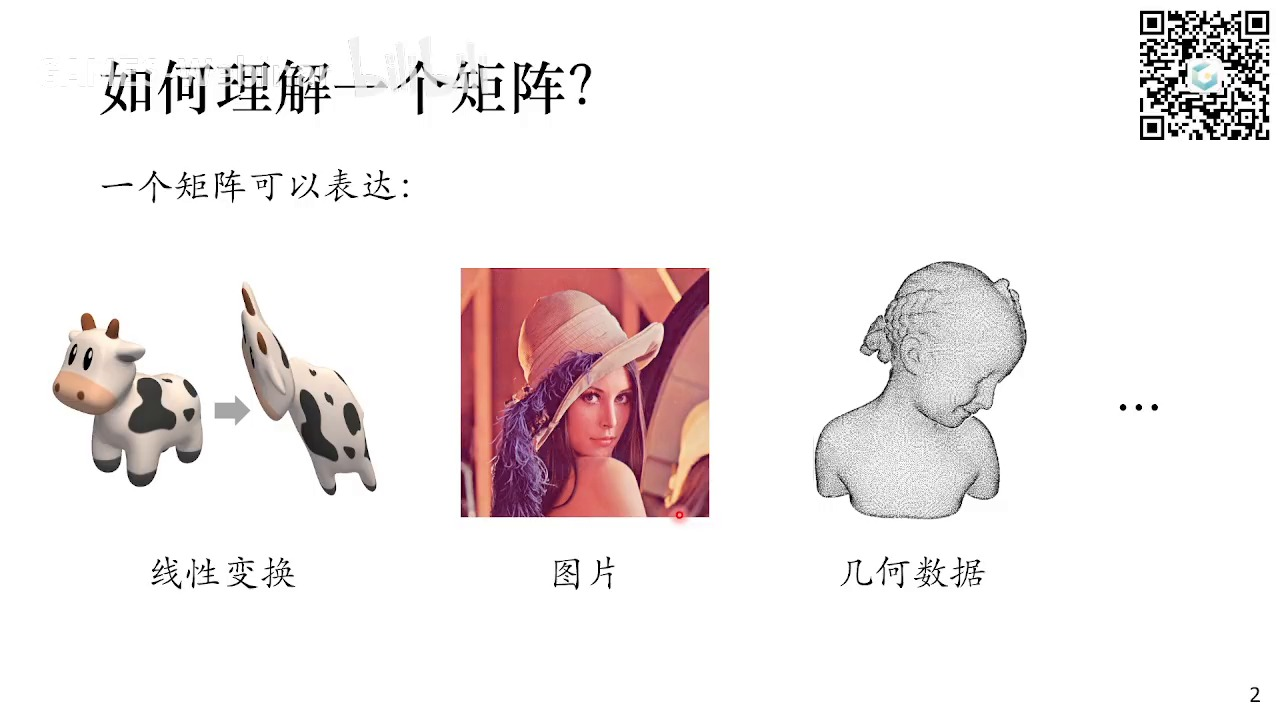
\includegraphics[width=0.92\textwidth]{figures/fig_01_matrix_meanings.jpg}
\caption{一个矩阵可以表达线性变换、图片和几何数据\vtag}
\end{figure}
\srcnote{00:01:30--00:01:45}
\end{minipage}


\noindent\begin{minipage}{\textwidth}
\begin{figure}[H]
\centering
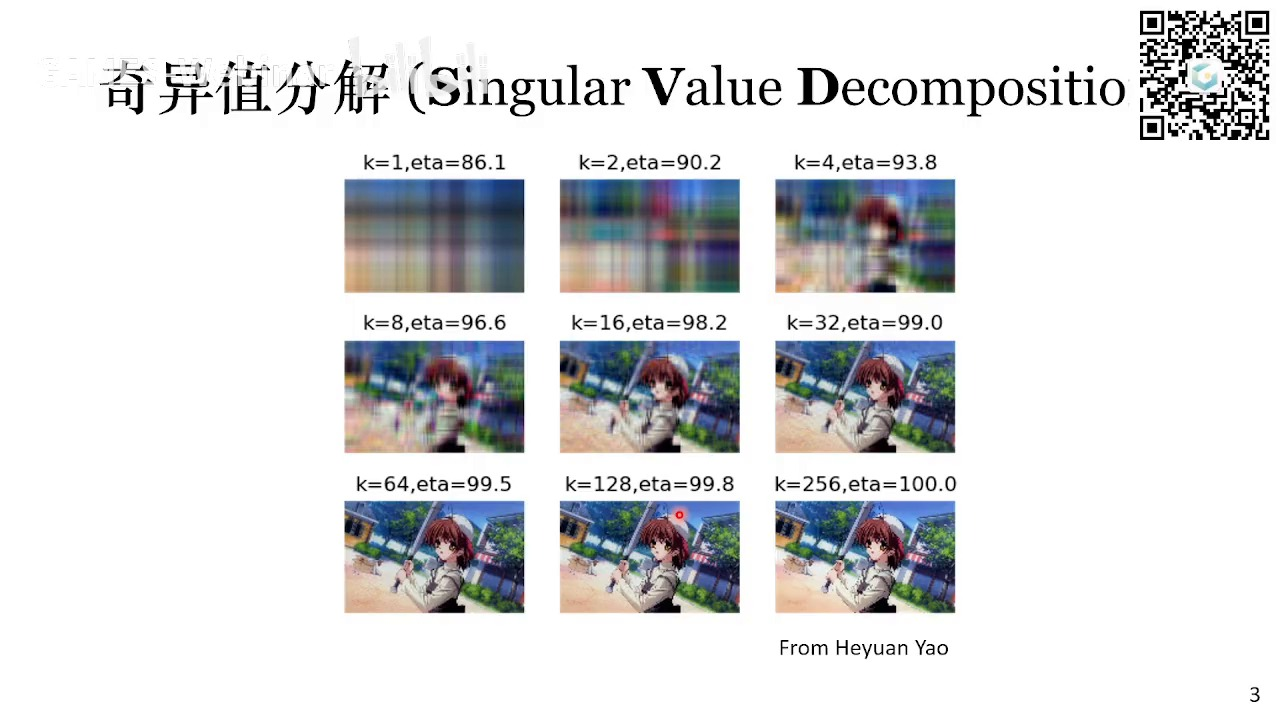
\includegraphics[width=0.92\textwidth]{figures/fig_02_svd_intro.jpg}
\caption{奇异值分解的直观演示：保留不同数量的奇异值，对图片做低秩近似\vtag}
\end{figure}
\srcnote{00:01:45--00:02:00}
\end{minipage}


\begin{importantbox}{本讲的主线}
本讲分两部分。第一部分从实对称矩阵的特征值分解出发推导 SVD，再用 SVD 统一处理矩阵的逆、伪逆、左逆与右逆，解释“旋转—拉伸—旋转”的几何意义与极分解，并介绍三个应用：形状匹配、图像压缩与 LoRA、SVD 的求导。第二部分介绍 PCA：从零阶、一阶近似一步步推出“主成分就是协方差矩阵的特征向量”，再看点云法向、Eigenfaces、模型降阶等应用，以及 PCA 在非线性数据上的局限。
\end{importantbox}

\section{实对称矩阵的特征值分解}

\subsection{两个定理}

SVD 建立在实对称矩阵的性质之上，讲者先证明两个定理。

\textbf{定理 1：实对称矩阵的特征值是实数。}设 $\mathrm S\mathbf x=\lambda\mathbf x$，其中 $\mathbf x$ 可以是复特征向量，并归一化为 $\mathbf x^{\mathsf T}\mathbf x^*=1$。对等式取共轭，由于 $\mathrm S$ 是实矩阵，$\mathrm S\mathbf x^*=\lambda^*\mathbf x^*$；两边左乘 $\mathbf x^{\mathsf T}$ 得 $\mathbf x^{\mathsf T}\mathrm S\mathbf x^*=\lambda^*$。另一方面，对原式取转置，由于 $\mathrm S^{\mathsf T}=\mathrm S$，$\mathbf x^{\mathsf T}\mathrm S=\lambda\mathbf x^{\mathsf T}$；两边右乘 $\mathbf x^*$ 得 $\mathbf x^{\mathsf T}\mathrm S\mathbf x^*=\lambda$。于是
\[
\lambda=\mathbf x^{\mathsf T}\mathrm S\mathbf x^*=\lambda^* ,
\]
特征值是实数。

\textbf{定理 2：实对称矩阵不同特征值的特征向量相互正交。}设 $\mathrm S\mathbf x_0=\lambda_0\mathbf x_0$，$\mathrm S\mathbf x_1=\lambda_1\mathbf x_1$，则
\[
\lambda_0\mathbf x_0^{\mathsf T}\mathbf x_1=\mathbf x_0^{\mathsf T}\mathrm S^{\mathsf T}\mathbf x_1=\mathbf x_0^{\mathsf T}\mathrm S\mathbf x_1=\lambda_1\mathbf x_0^{\mathsf T}\mathbf x_1 .
\]
若 $\lambda_0\neq\lambda_1$，只能 $\mathbf x_0^{\mathsf T}\mathbf x_1=0$。

\noindent\begin{minipage}{\textwidth}
\begin{figure}[H]
\centering
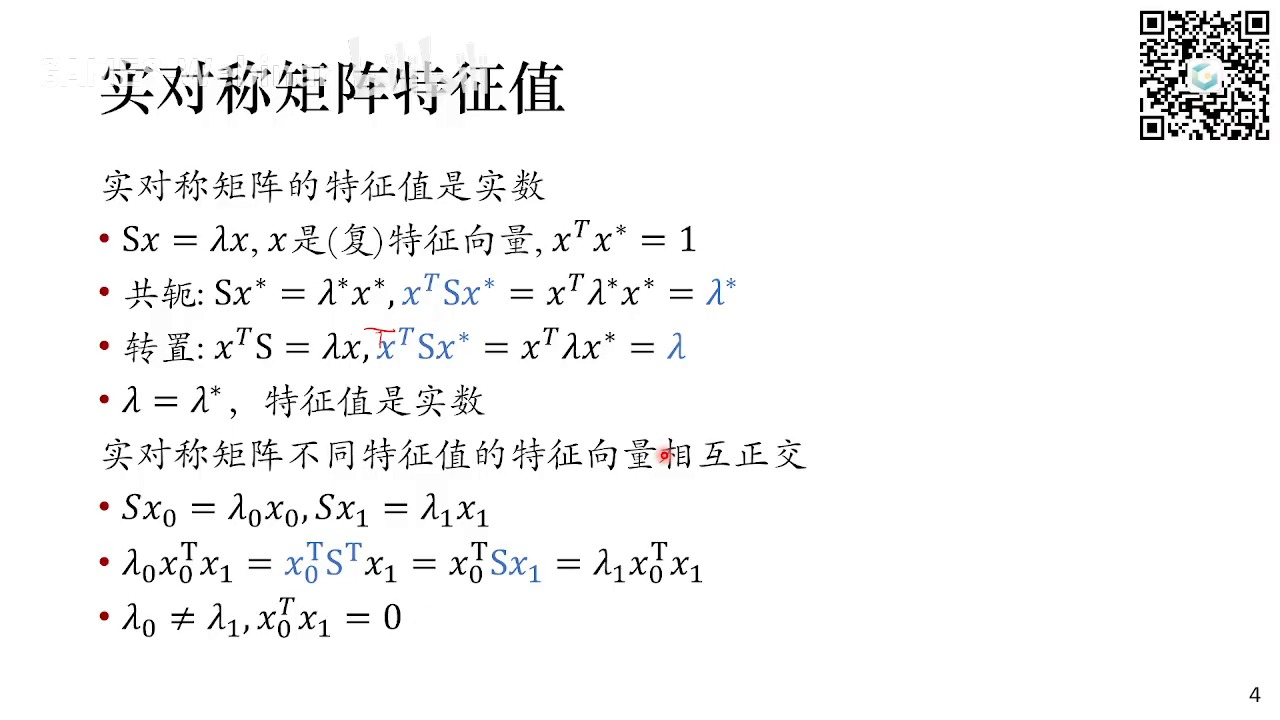
\includegraphics[width=0.92\textwidth]{figures/fig_03_sym_eig.jpg}
\caption{实对称矩阵的两个定理：特征值为实数，不同特征值的特征向量正交\vtag}
\end{figure}
\srcnote{00:06:45--00:07:00}
\end{minipage}


\subsection{特征值分解与半正定矩阵}

由这两个定理（重特征值的特征子空间内可以再做正交化），任意实对称矩阵都能写成
\[
\mathrm S=\mathrm Q\Lambda\mathrm Q^{\mathsf T}=
\begin{pmatrix}\mathbf q_0&\cdots&\mathbf q_{n-1}\end{pmatrix}
\begin{pmatrix}\lambda_0&&\\&\ddots&\\&&\lambda_{n-1}\end{pmatrix}
\begin{pmatrix}\mathbf q_0^{\mathsf T}\\ \vdots\\ \mathbf q_{n-1}^{\mathsf T}\end{pmatrix},\qquad \mathrm Q^{\mathsf T}\mathrm Q=\mathrm I .
\]
特征值 $\lambda_i$ 有正有负；当 $\mathrm S$ 的秩为 $r$ 时，只有 $r$ 个 $\lambda_i$ 非零。

如果所有 $\lambda_i$ 都非负，$\mathrm S$ 就是半正定矩阵（课件记为 SPD，semi positive definite）。用特征值分解可以直接验证二次型非负：
\[
\mathbf x^{\mathsf T}\mathrm S\mathbf x=\mathbf x^{\mathsf T}\mathrm Q\Lambda\mathrm Q^{\mathsf T}\mathbf x=\|\mathrm Q^{\mathsf T}\mathbf x\|_\Lambda^2=\sum_i\lambda_i(\mathbf q_i^{\mathsf T}\mathbf x)^2\ge0 .
\]
对半正定矩阵还可以定义实对角矩阵 $\Sigma$，满足 $\Sigma^2=\Lambda$，于是
\[
\mathrm S=\mathrm Q\Sigma^2\mathrm Q^{\mathsf T}=(\mathrm Q\Sigma\mathrm Q^{\mathsf T})(\mathrm Q\Sigma\mathrm Q^{\mathsf T})=\mathrm P^2
\;\Longrightarrow\;\mathrm P=\mathrm S^{1/2}.
\]
中间插入 $\mathrm Q^{\mathsf T}\mathrm Q=\mathrm I$ 是这里的关键技巧。讲者说这是实对称半正定矩阵另一个非常有用的性质：它总有一个“平方根”，而且平方根本身也是对称半正定的。后面形状匹配中证明迹不等式时，用的正是这个平方根。最后，迹在循环置换下不变，所以
\[
\operatorname{Tr}\mathrm S=\operatorname{Tr}(\mathrm Q\Lambda\mathrm Q^{\mathsf T})=\operatorname{Tr}(\mathrm Q^{\mathsf T}\mathrm Q\Lambda)=\operatorname{Tr}\Lambda=\sum_i\lambda_i .
\]

\noindent\begin{minipage}{\textwidth}
\begin{figure}[H]
\centering
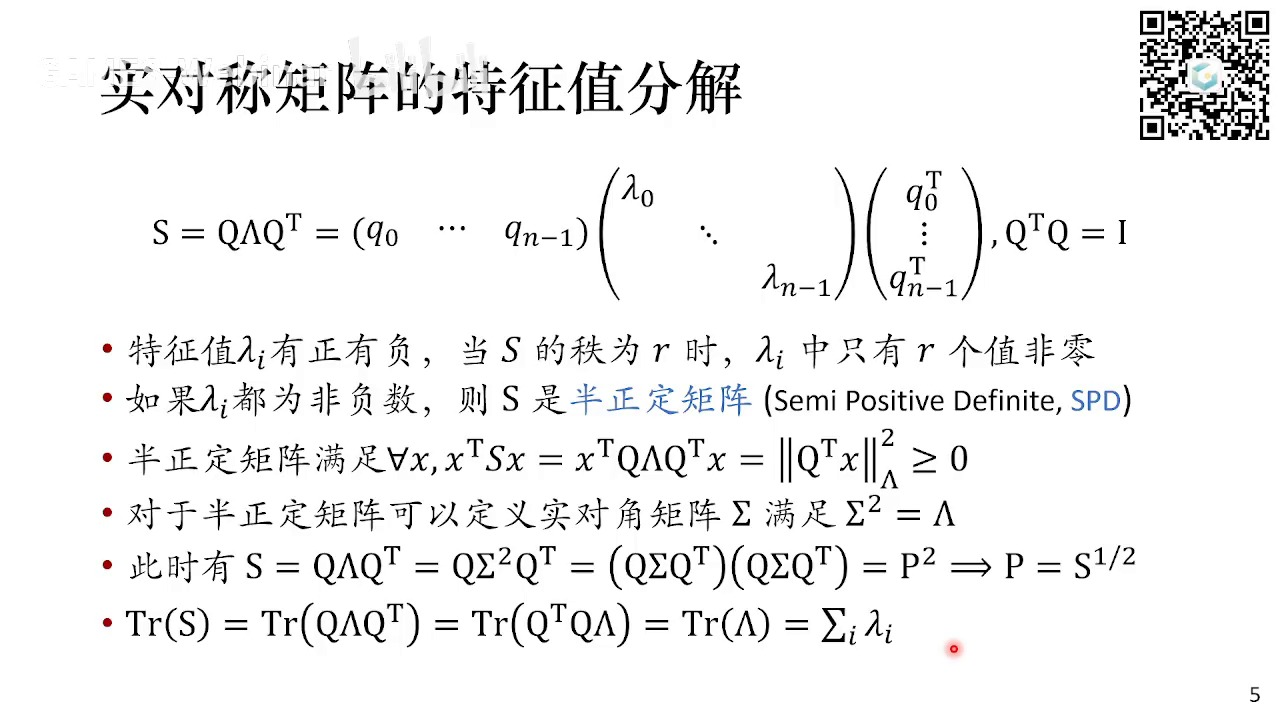
\includegraphics[width=0.92\textwidth]{figures/fig_04_sym_eigdecomp.jpg}
\caption{实对称矩阵的特征值分解、半正定矩阵的平方根与迹\vtag}
\end{figure}
\srcnote{00:13:45--00:14:00}
\end{minipage}


\begin{warningbox}{缩写 SPD 的两种含义}
课件把半正定矩阵缩写为 SPD（semi positive definite）。讲义作者提醒：大多数文献中 SPD 指“对称正定”（symmetric positive definite），半正定通常写作 PSD 或 SPSD。阅读其它资料时要留意上下文。
\end{warningbox}

\section{奇异值分解}

\subsection{从 $\mathrm A^{\mathsf T}\mathrm A$ 推出 SVD}

对任意矩阵 $\mathrm A\in\mathbb R^{m\times n}$，它不一定是方阵，设其秩为 $r$。矩阵 $\mathrm S=\mathrm A^{\mathsf T}\mathrm A$ 是对称半正定的，因为 $\mathbf x^{\mathsf T}\mathrm A^{\mathsf T}\mathrm A\mathbf x=\|\mathrm A\mathbf x\|^2\ge0$。于是可以找到特征对
\[
\mathrm A^{\mathsf T}\mathrm A\mathbf v_i=\lambda_i\mathbf v_i,\qquad
\mathbf v_i^{\mathsf T}\mathrm A^{\mathsf T}\mathrm A\mathbf v_j=\lambda_j\mathbf v_i^{\mathsf T}\mathbf v_j=\lambda_j\delta_{ij},
\]
$\{\mathbf v_i\}$ 是一组 $r$ 个正交基。定义
\[
\mathbf u_i=\frac{1}{\sqrt{\lambda_i}}\mathrm A\mathbf v_i ,
\]
则 $\mathbf u_i^{\mathsf T}\mathbf u_j=\delta_{ij}$，$\{\mathbf u_i\}$ 也是一组 $r$ 个正交基。再用施密特正交化把 $\mathbf v_i$ 扩充为 $\mathbb R^n$ 的 $n$ 个正交基、把 $\mathbf u_i$ 扩充为 $\mathbb R^m$ 的 $m$ 个正交基；扩充的基满足 $\sqrt{\lambda_j}\mathbf u_j=\mathbf 0=\mathrm A\mathbf v_j$。把 $\sqrt{\lambda_i}\mathbf u_i=\mathrm A\mathbf v_i$ 写成矩阵，得到 $\mathrm A\mathrm V=\mathrm U\Sigma$，右乘 $\mathrm V^{\mathsf T}$ 就是
\[
\mathrm A=\mathrm U\Sigma\mathrm V^{\mathsf T},\qquad
\Sigma_{ii}=\begin{cases}\sqrt{\lambda_i},&i\le r\\0,&i>r\end{cases}
\]
其中 $\mathrm U\in\mathbb R^{m\times m}$、$\mathrm V\in\mathbb R^{n\times n}$ 是正交矩阵，$\Sigma\in\mathbb R^{m\times n}$ 是“对角”矩阵：它不是方阵，但仍可以定义对角元。

把这段推导串起来看，思路其实很清楚。第一步，任意矩阵本身没有好的性质，但 $\mathrm A^{\mathsf T}\mathrm A$ 是对称半正定的，可以用上一节的定理做正交对角化，得到右侧的一组正交基 $\mathbf v_i$。第二步，用 $\mathrm A$ 把这组基映射过去，再除以长度 $\sqrt{\lambda_i}$，得到左侧的一组正交基 $\mathbf u_i$；它们之所以正交，正是因为 $\mathbf v_i$ 是 $\mathrm A^{\mathsf T}\mathrm A$ 的特征向量。第三步，秩为 $r$ 时只能得到 $r$ 对向量，于是用施密特正交化把两边都补齐；补上的向量对应的特征值为零，所以原来的关系 $\sqrt{\lambda_j}\mathbf u_j=\mathrm A\mathbf v_j$ 对它们同样成立，两边都等于零。最后把所有列排成矩阵，就离 SVD 只差“右乘 $\mathrm V^{\mathsf T}$”这一步。

\noindent\begin{minipage}{\textwidth}
\begin{figure}[H]
\centering
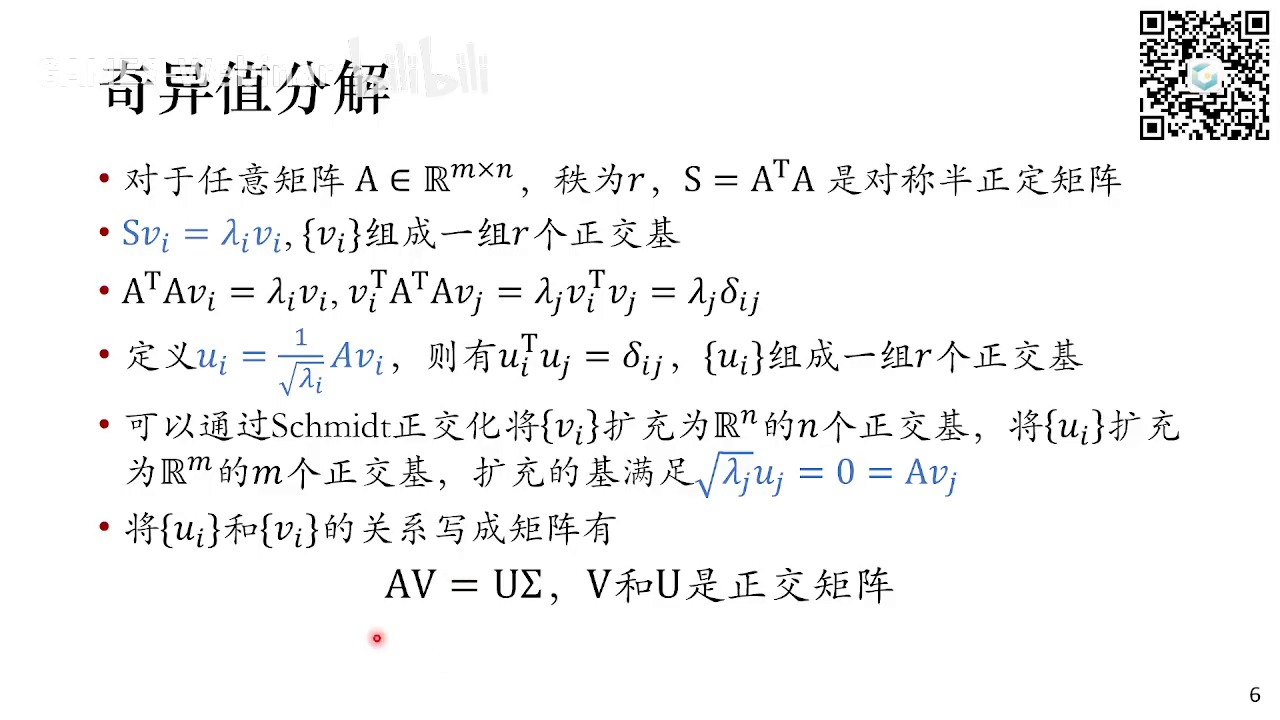
\includegraphics[width=0.92\textwidth]{figures/fig_05_svd_derive.jpg}
\caption{SVD 的推导：$\mathrm A^{\mathsf T}\mathrm A$ 的特征向量给出 $\mathbf v_i$，$\mathbf u_i=\mathrm A\mathbf v_i/\sqrt{\lambda_i}$\vtag}
\end{figure}
\srcnote{00:21:15--00:21:30}
\end{minipage}


\noindent\begin{minipage}{\textwidth}
\begin{figure}[H]
\centering
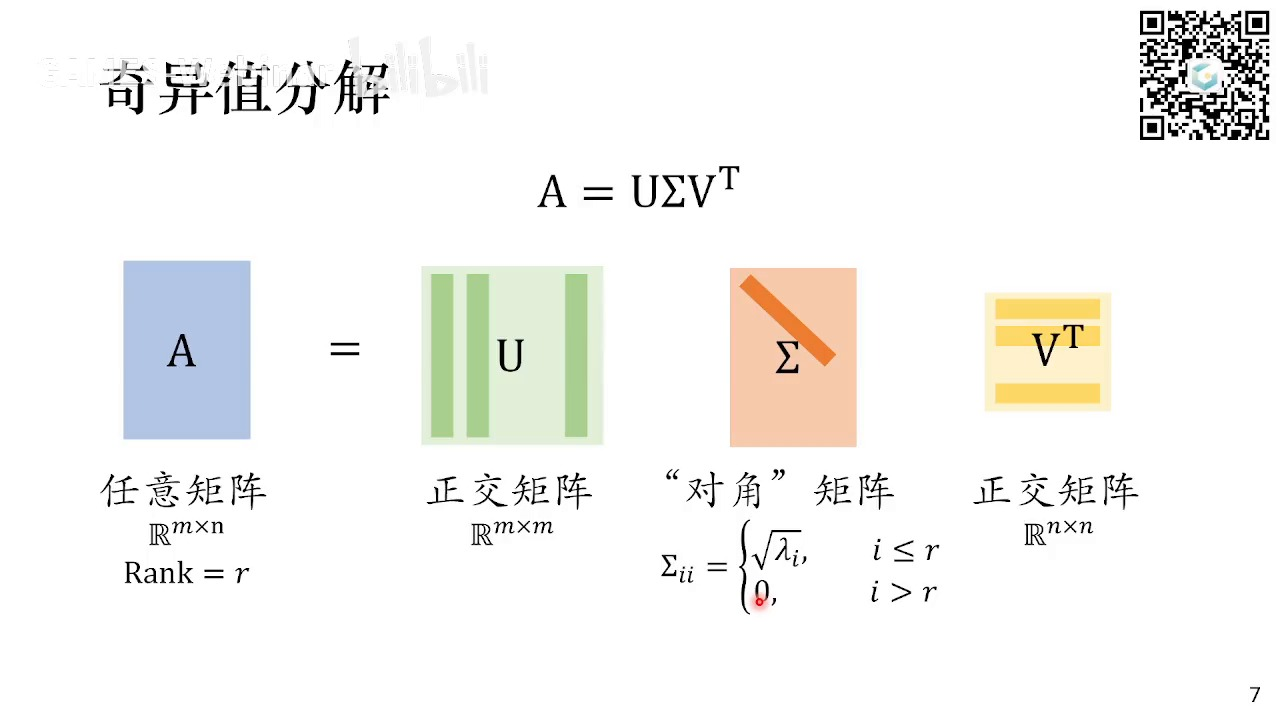
\includegraphics[width=0.92\textwidth]{figures/fig_06_svd_form.jpg}
\caption{SVD 的形式：任意矩阵 $=$ 正交矩阵 $\times$ “对角”矩阵 $\times$ 正交矩阵\vtag}
\end{figure}
\srcnote{00:23:45--00:24:00}
\end{minipage}


讲者说，前面的推导如果没有完全理解也没关系，但这个形式对线性代数非常重要，一定要记住。弹幕中有同学问奇异值的个数是否不超过秩：奇异值中非零的个数恰好等于矩阵的秩 $r$；它们由开根号定义，所以一定是正的，其余对角元为零。

讲者特别强调这个形式之所以重要，是因为它非常“朴实”：任意矩阵 $\mathrm A$，不必是方阵，也不必满秩，都可以写成 $\mathrm U\Sigma\mathrm V^{\mathsf T}$ 的形式，其中两边是正交矩阵，中间是类似对角矩阵的东西。后面所有的应用，无论求逆、求最小二乘解，还是做形状匹配、图像压缩，都是把问题放到 $\mathrm U$ 和 $\mathrm V$ 定义的坐标系里，在那里矩阵只剩下对角的缩放，问题就变得几乎一目了然。

\begin{knowledgebox}{SVD 与特征值分解的区别}
特征值分解 $\mathrm S=\mathrm Q\Lambda\mathrm Q^{\mathsf T}$ 只对方阵有意义，而且只有实对称矩阵才保证能用正交矩阵对角化，特征值也可能为负。SVD 对任意 $m\times n$ 矩阵都存在，左右两侧用的是两组不同的正交基 $\mathrm U$ 和 $\mathrm V$，奇异值总是非负的。两者的联系就是本节的推导：$\mathrm A$ 的右奇异向量是 $\mathrm A^{\mathsf T}\mathrm A$ 的特征向量，左奇异向量是 $\mathrm A\mathrm A^{\mathsf T}$ 的特征向量，奇异值是对应特征值的平方根。对实对称半正定矩阵，两种分解完全重合。
\end{knowledgebox}

\subsection{SVD 能告诉我们什么}

SVD 是线性代数中非常重要的概念，在图形学中应用广泛。已知一个矩阵的 SVD，可以直接得到：矩阵的逆（求解矩阵方程）、矩阵的秩、矩阵方程的最小二乘解、极分解等等。

\noindent\begin{minipage}{\textwidth}
\begin{figure}[H]
\centering
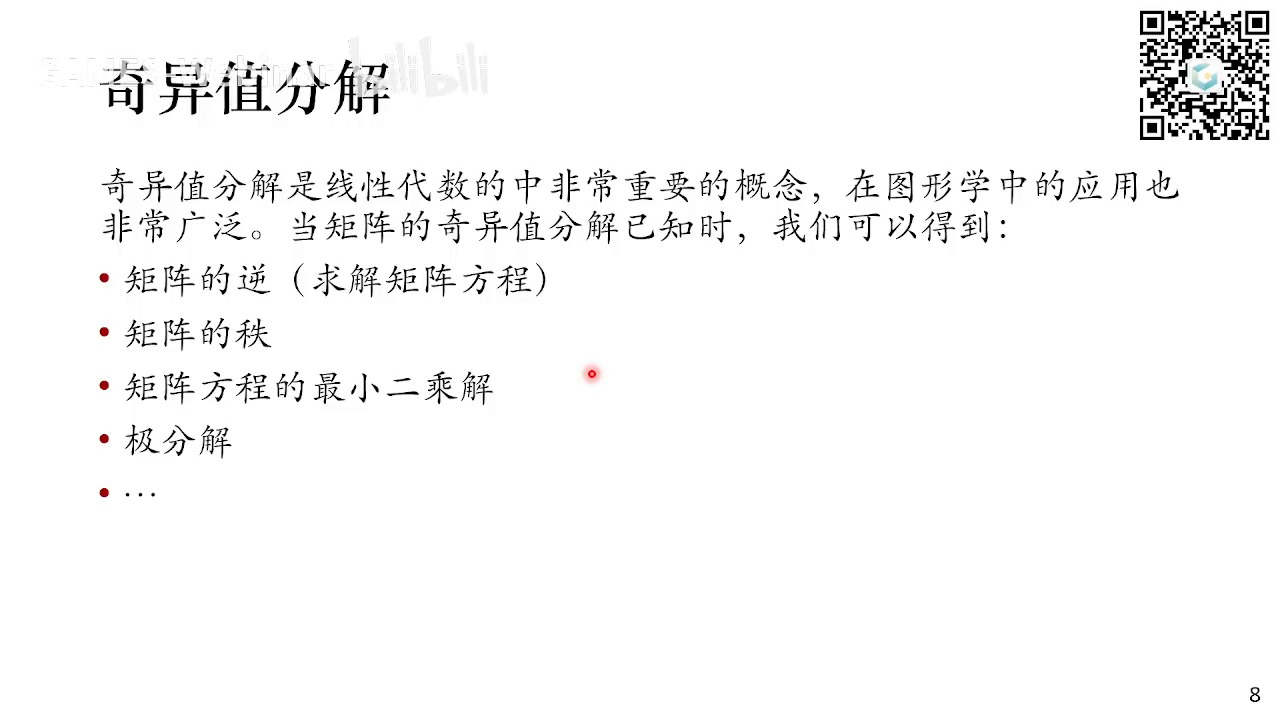
\includegraphics[width=0.92\textwidth]{figures/fig_07_svd_uses.jpg}
\caption{已知 SVD 时可以得到的东西：逆、秩、最小二乘解、极分解\vtag}
\end{figure}
\srcnote{00:24:15--00:24:30}
\end{minipage}


\section{逆、伪逆、左逆与右逆}

\subsection{可逆矩阵的逆}

对可逆矩阵 $\mathrm A\in\mathbb R^{n\times n}$，$\mathrm A=\mathrm U\Sigma\mathrm V^{\mathsf T}$。由于正交矩阵的逆是转置，
\[
\mathrm A^{-1}=(\mathrm U\Sigma\mathrm V^{\mathsf T})^{-1}=\mathrm V\Sigma^{-1}\mathrm U^{\mathsf T}
=\mathrm V\begin{pmatrix}1/\sigma_0&&\\&\ddots&\\&&1/\sigma_{n-1}\end{pmatrix}\mathrm U^{\mathsf T}.
\]

\noindent\begin{minipage}{\textwidth}
\begin{figure}[H]
\centering
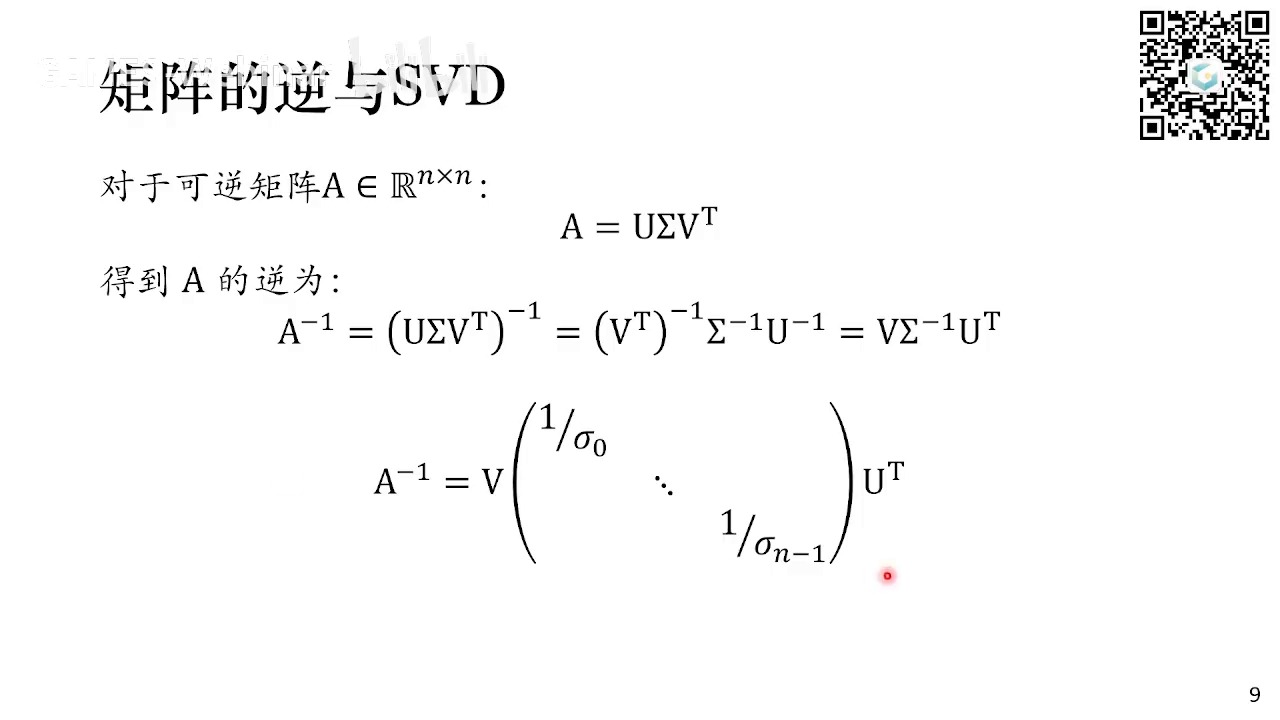
\includegraphics[width=0.92\textwidth]{figures/fig_08_inverse.jpg}
\caption{可逆矩阵的逆：$\mathrm A^{-1}=\mathrm V\Sigma^{-1}\mathrm U^{\mathsf T}$\vtag}
\end{figure}
\srcnote{00:25:45--00:26:00}
\end{minipage}


\subsection{超定方程与伪逆}

SVD 的威力在于它对任意矩阵都成立。考虑 $\mathrm A\mathbf x=\mathbf b$，$\mathrm A\in\mathbb R^{m\times n}$ 列满秩但 $m>n$：方程个数 $m$ 大于自由度个数 $n$，解不一定存在，这是\textbf{超定}情况。讲者描述这种矩阵的样子是“很长的”：行很多、列很少，例如用大量测量数据去拟合少数几个参数。此时寻找最小二乘解
\[
\min_{\mathbf x}\|\mathrm A\mathbf x-\mathbf b\|^2 .
\]
代入 SVD，并利用正交矩阵不改变长度：
\[
\|\mathrm A\mathbf x-\mathbf b\|^2=\|\mathrm U(\Sigma\mathrm V^{\mathsf T}\mathbf x-\mathrm U^{\mathsf T}\mathbf b)\|^2=\|\Sigma\mathbf x'-\mathbf b'\|^2,\qquad
\mathbf x'=\mathrm V^{\mathsf T}\mathbf x,\ \mathbf b'=\mathrm U^{\mathsf T}\mathbf b .
\]
$\Sigma\mathbf x'=(\sigma_0x'_0,\dots,\sigma_{n-1}x'_{n-1},0,0,\dots)$。后面 $m-n$ 项全是零，无论怎么改变 $\mathbf x'$ 都改变不了，只能不管；这一部分残差就是最小二乘解无法消除的误差；前 $n$ 项可以让残差为零：$\sigma_ix'_i=b'_i$。于是 $\mathbf x'=\hat\Sigma^{-1}\mathbf b'$，乘回去得到
\[
\mathbf x=\mathrm V\hat\Sigma^{-1}\mathrm U^{\mathsf T}\mathbf b .
\]
$\mathrm V\hat\Sigma^{-1}\mathrm U^{\mathsf T}$ 称为矩阵的\textbf{伪逆}（pseudo inverse）。$\hat\Sigma^{-1}$ 是 $n\times m$ 矩阵，形状与 $\Sigma^{\mathsf T}$ 相同，对角元为 $1/\sigma_i$。

\noindent\begin{minipage}{\textwidth}
\begin{figure}[H]
\centering
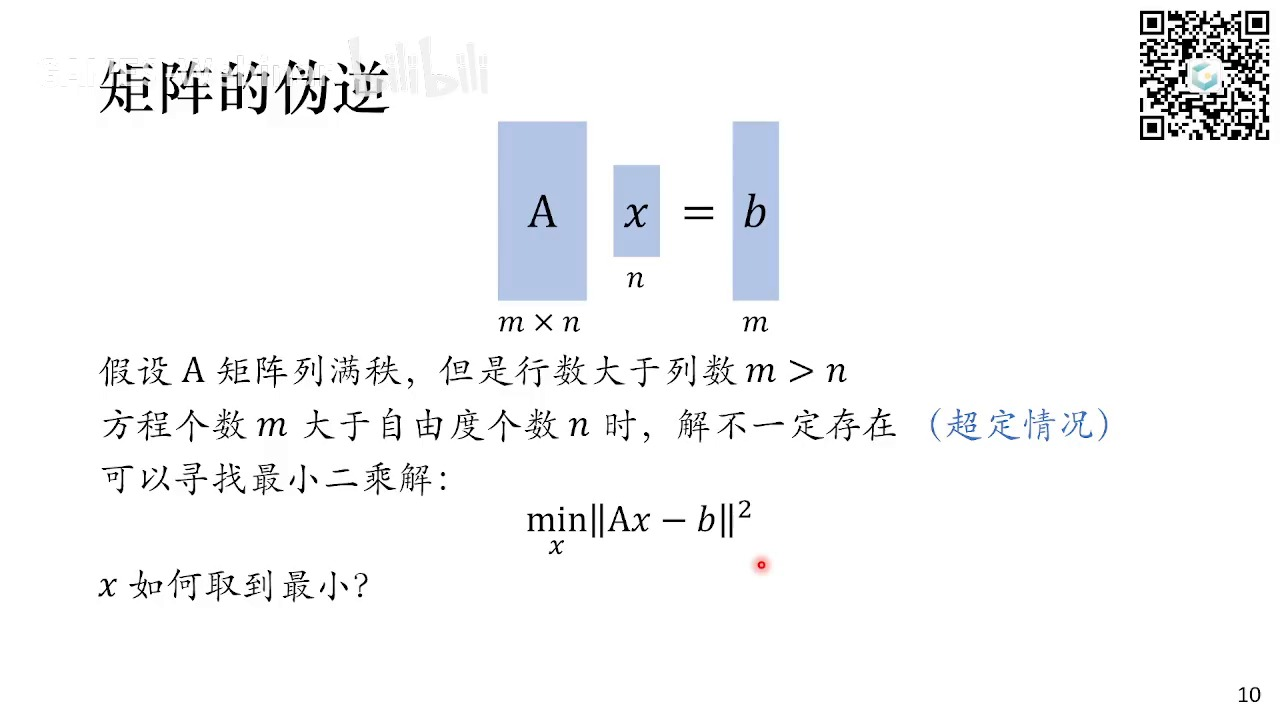
\includegraphics[width=0.92\textwidth]{figures/fig_09_pseudo_setup.jpg}
\caption{超定方程 $m>n$：解不一定存在，寻找最小二乘解\vtag}
\end{figure}
\srcnote{00:27:45--00:28:00}
\end{minipage}


\noindent\begin{minipage}{\textwidth}
\begin{figure}[H]
\centering
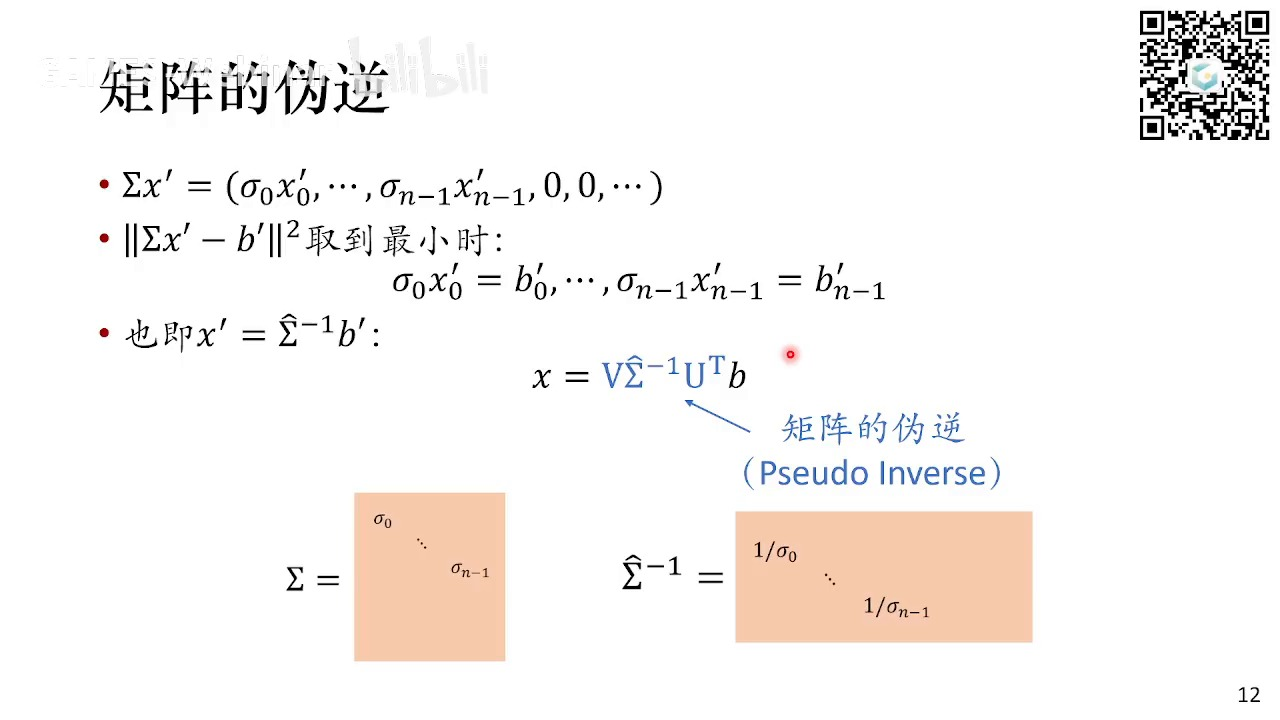
\includegraphics[width=0.92\textwidth]{figures/fig_10_pseudo_inverse.jpg}
\caption{在 $\mathbf x'=\mathrm V^{\mathsf T}\mathbf x$ 坐标下求最小二乘解，得到伪逆 $\mathrm V\hat\Sigma^{-1}\mathrm U^{\mathsf T}$\vtag}
\end{figure}
\srcnote{00:34:15--00:34:30}
\end{minipage}


\subsection{从矩阵求导推出左逆}

同一个问题也可以用第二讲的矩阵求导来解。展开
\[
g=\|\mathrm A\mathbf x-\mathbf b\|^2=\mathbf x^{\mathsf T}\mathrm A^{\mathsf T}\mathrm A\mathbf x-\mathbf x^{\mathsf T}\mathrm A^{\mathsf T}\mathbf b-\mathbf b^{\mathsf T}\mathrm A\mathbf x+\mathbf b^{\mathsf T}\mathbf b,\qquad
\frac{\partial g}{\partial\mathbf x}=2\mathrm A^{\mathsf T}\mathrm A\mathbf x-2\mathrm A^{\mathsf T}\mathbf b=0 .
\]
$g$ 是关于 $\mathbf x$ 的二次函数，导数为零处取最小值，得到正规方程 $\mathrm A^{\mathsf T}\mathrm A\mathbf x=\mathrm A^{\mathsf T}\mathbf b$。$\mathrm A$ 是又高又瘦的矩阵，$\mathrm A^{\mathsf T}\mathrm A\in\mathbb R^{n\times n}$ 却是满秩方阵，所以（$\mathrm A^{\mathsf T}$ 是又矮又宽的矩阵，二者相乘回到 $n\times n$；又因为 $\mathrm A$ 列满秩，乘积也满秩）
\[
\mathbf x=(\mathrm A^{\mathsf T}\mathrm A)^{-1}\mathrm A^{\mathsf T}\mathbf b .
\]
$(\mathrm A^{\mathsf T}\mathrm A)^{-1}\mathrm A^{\mathsf T}$ 称为\textbf{左逆}（left inverse），因为它乘在 $\mathrm A$ 左边得到单位阵，乘在右边则不是：$(\mathrm A^{\mathsf T}\mathrm A)^{-1}\mathrm A^{\mathsf T}\mathrm A=\mathrm I$，$\mathrm A(\mathrm A^{\mathsf T}\mathrm A)^{-1}\mathrm A^{\mathsf T}\neq\mathrm I$。

\noindent\begin{minipage}{\textwidth}
\begin{figure}[H]
\centering
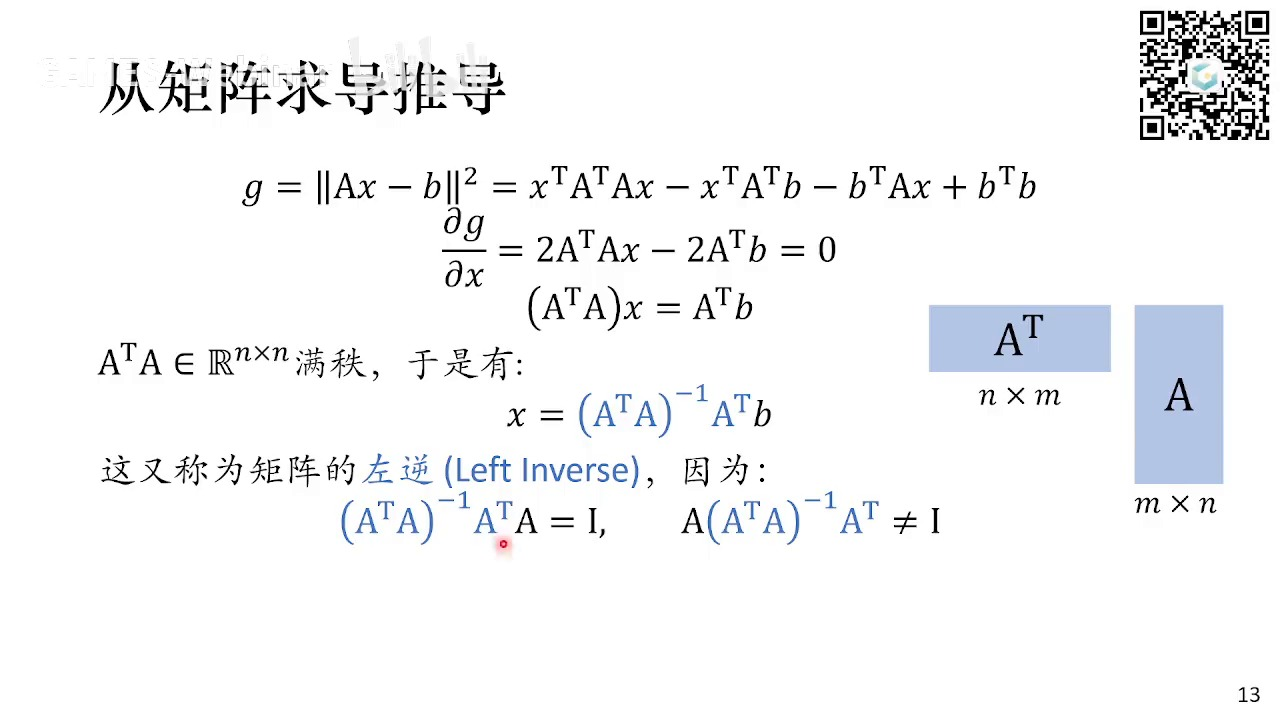
\includegraphics[width=0.92\textwidth]{figures/fig_11_left_inverse.jpg}
\caption{从矩阵求导得到正规方程与左逆\vtag}
\end{figure}
\srcnote{00:37:15--00:37:30}
\end{minipage}


左逆与伪逆是什么关系？代入 SVD，$\mathrm A^{\mathsf T}\mathrm A=\mathrm V\Sigma^{\mathsf T}\Sigma\mathrm V^{\mathsf T}=\mathrm V\Lambda\mathrm V^{\mathsf T}$，于是
\[
(\mathrm A^{\mathsf T}\mathrm A)^{-1}\mathrm A^{\mathsf T}=\mathrm V\Lambda^{-1}\mathrm V^{\mathsf T}\mathrm V\Sigma^{\mathsf T}\mathrm U^{\mathsf T}=\mathrm V\Lambda^{-1}\Sigma^{\mathsf T}\mathrm U^{\mathsf T}=\mathrm V\hat\Sigma^{-1}\mathrm U^{\mathsf T}.
\]
$\Lambda^{-1}\Sigma^{\mathsf T}$ 的对角元是 $\sigma_i/\sigma_i^2=1/\sigma_i$。所以矩阵列满秩时，左逆与伪逆等价。

\noindent\begin{minipage}{\textwidth}
\begin{figure}[H]
\centering
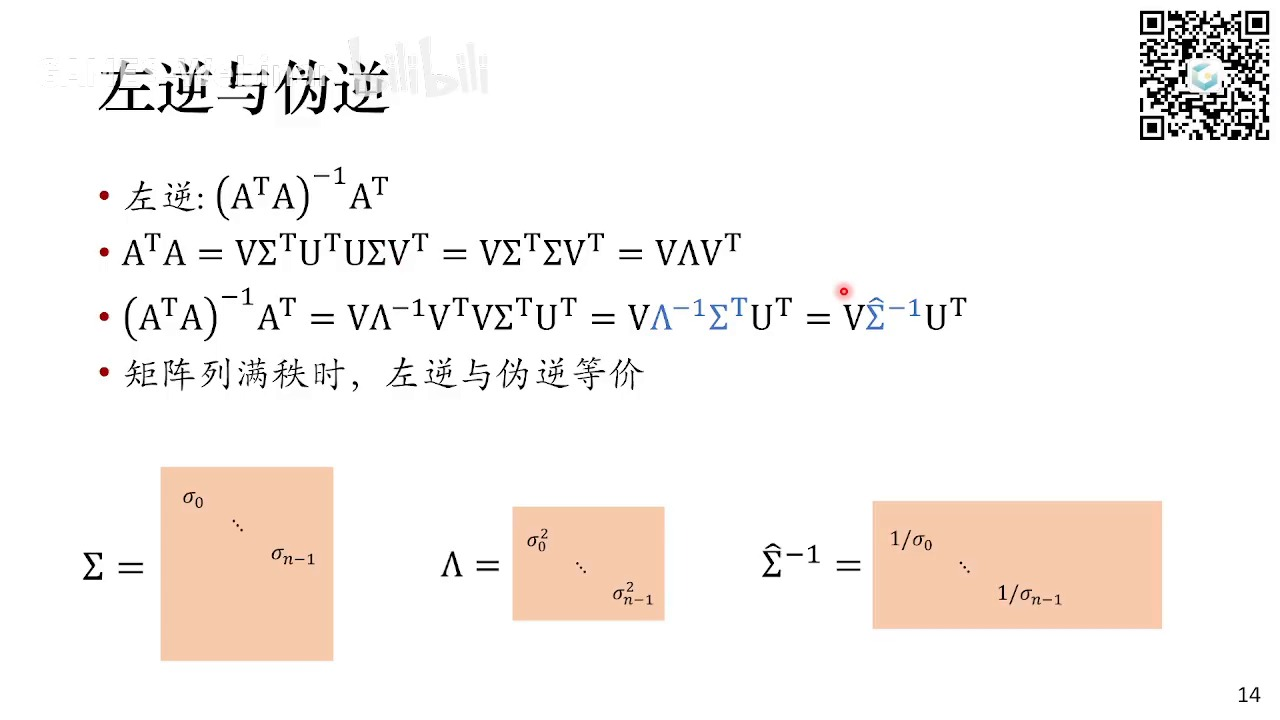
\includegraphics[width=0.92\textwidth]{figures/fig_12_left_pseudo.jpg}
\caption{列满秩时左逆与伪逆等价\vtag}
\end{figure}
\srcnote{00:39:30--00:39:45}
\end{minipage}


\subsection{欠定方程与右逆}

另一种情况是 $\mathrm A$ 行满秩但 $m<n$：自由度个数大于方程个数，有无穷多组解，这是\textbf{欠定}情况。此时寻求范数最小的解：
\[
\min_{\mathbf x}\|\mathbf x\|^2\quad\text{s.t.}\quad\mathrm A\mathbf x-\mathbf b=0 .
\]
同样换到 $\mathbf x'=\mathrm V^{\mathsf T}\mathbf x$，$\mathbf b'=\mathrm U^{\mathsf T}\mathbf b$ 坐标，约束变为 $\Sigma\mathbf x'=\mathbf b'$，即 $\sigma_ix'_i=b'_i$，$i=0,\dots,m-1$；剩下的 $x'_m,\dots,x'_{n-1}$ 可以取任意值。由于 $\|\mathbf x'\|^2=\mathbf x^{\mathsf T}\mathrm V\mathrm V^{\mathsf T}\mathbf x=\|\mathbf x\|^2$，要让 $\|\mathbf x\|$ 最小，就令这些自由分量全为零。讲者在这里点出了与超定情况的区别：欠定时残差总能取到零，所以“最小二乘”不再指残差最小，而是指在所有满足方程的解中，选模长最小的那一个。结果仍然是
\[
\mathbf x'=\hat\Sigma^{-1}\mathbf b',\qquad \mathbf x=\mathrm V\hat\Sigma^{-1}\mathrm U^{\mathsf T}\mathbf b .
\]

\noindent\begin{minipage}{\textwidth}
\begin{figure}[H]
\centering
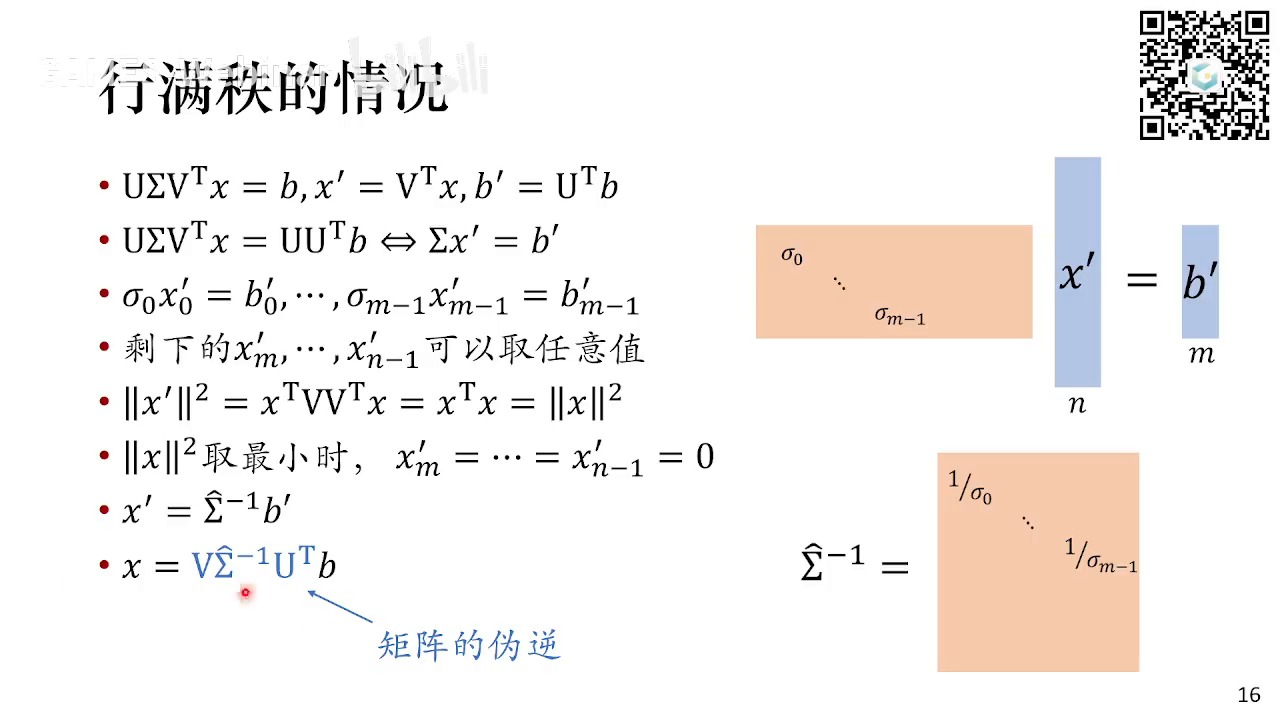
\includegraphics[width=0.92\textwidth]{figures/fig_13_row_full.jpg}
\caption{行满秩的欠定方程：自由分量取零得到最小范数解，结果仍是伪逆\vtag}
\end{figure}
\srcnote{00:44:30--00:44:45}
\end{minipage}


利用 $\hat\Sigma^{-1}=\Sigma^{\mathsf T}(\Sigma\Sigma^{\mathsf T})^{-1}$，可以把伪逆写成
\[
\mathrm V\hat\Sigma^{-1}\mathrm U^{\mathsf T}=\mathrm A^{\mathsf T}(\mathrm A\mathrm A^{\mathsf T})^{-1},
\]
称为\textbf{右逆}（right inverse）：$\mathrm A\mathrm A^{\mathsf T}(\mathrm A\mathrm A^{\mathsf T})^{-1}=\mathrm I$，而 $\mathrm A^{\mathsf T}(\mathrm A\mathrm A^{\mathsf T})^{-1}\mathrm A\neq\mathrm I$。直接求解这个带约束的优化问题需要拉格朗日乘子法，后面的最优化课程会介绍。

\noindent\begin{minipage}{\textwidth}
\begin{figure}[H]
\centering
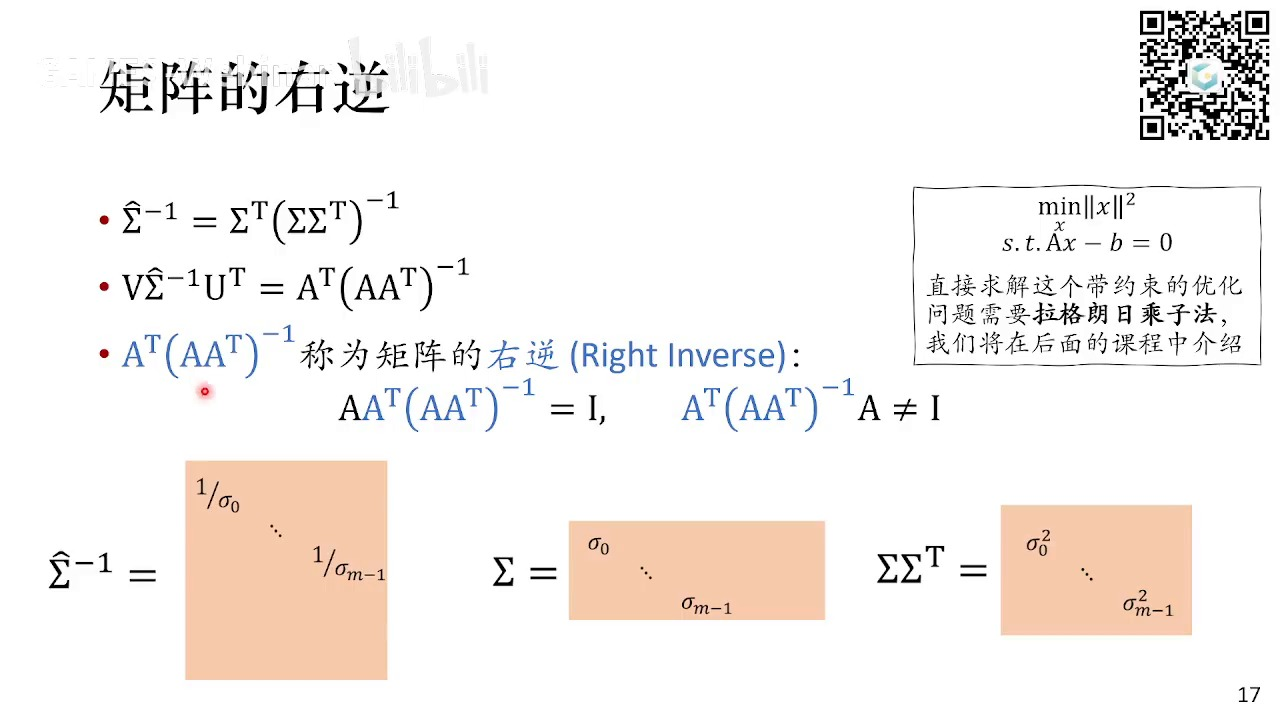
\includegraphics[width=0.92\textwidth]{figures/fig_14_right_inverse.jpg}
\caption{右逆 $\mathrm A^{\mathsf T}(\mathrm A\mathrm A^{\mathsf T})^{-1}$\vtag}
\end{figure}
\srcnote{00:47:00--00:47:15}
\end{minipage}


\begin{importantbox}{左逆、右逆、伪逆}
\begin{itemize}
\item 矩阵列满秩时，左逆 $(\mathrm A^{\mathsf T}\mathrm A)^{-1}\mathrm A^{\mathsf T}$ 存在，用于求解超定方程，给出残差最小的解。
\item 矩阵行满秩时，右逆 $\mathrm A^{\mathsf T}(\mathrm A\mathrm A^{\mathsf T})^{-1}$ 存在，用于求解欠定方程，给出范数最小的解。
\item 不管什么情况，伪逆 $\mathrm V\hat\Sigma^{-1}\mathrm U^{\mathsf T}$ 一定存在。秩亏时只对非零奇异值取倒数，零奇异值对应位置保持为零。
\end{itemize}
\end{importantbox}

\noindent\begin{minipage}{\textwidth}
\begin{figure}[H]
\centering
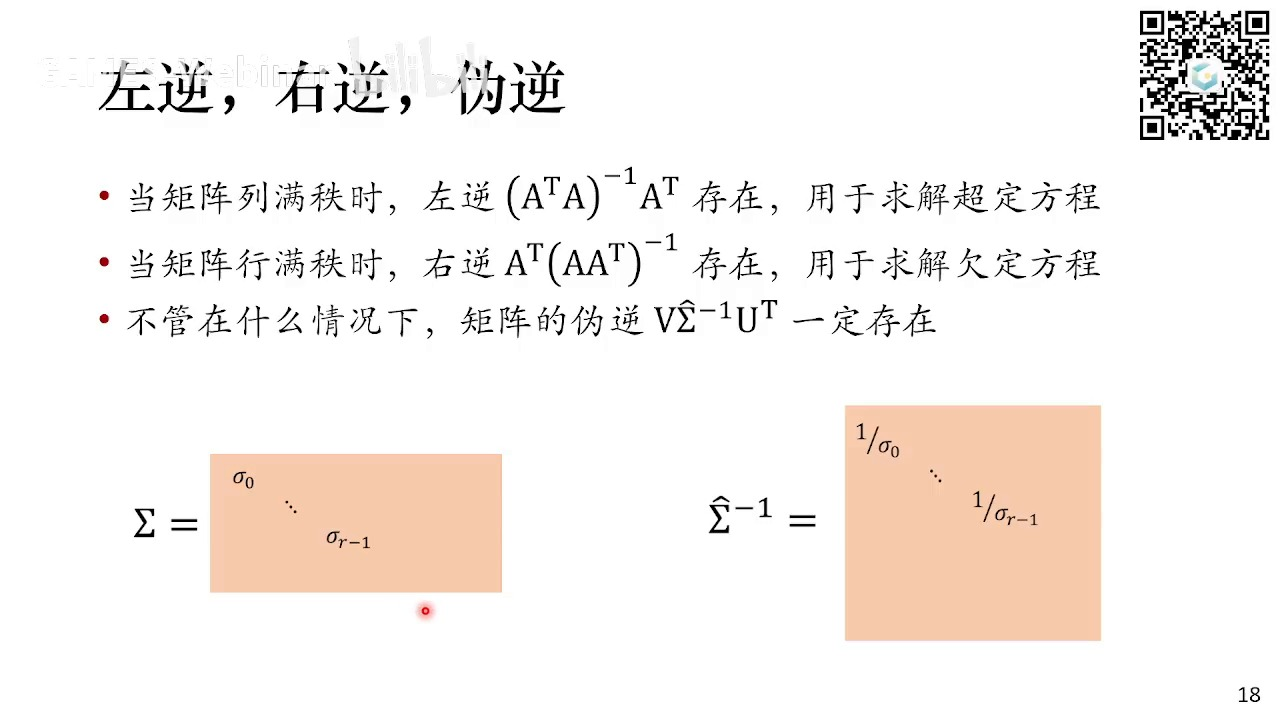
\includegraphics[width=0.92\textwidth]{figures/fig_15_three_inverses.jpg}
\caption{左逆、右逆、伪逆的总结\vtag}
\end{figure}
\srcnote{00:50:00--00:50:15}
\end{minipage}


\section{SVD 的几何意义与极分解}

\subsection{旋转—拉伸—旋转}

$\mathbf x'\leftarrow\mathrm A\mathbf x=\mathrm U\Sigma\mathrm V^{\mathsf T}\mathbf x$ 可以拆成三步：先 $\mathbf x'\leftarrow\mathrm V^{\mathsf T}\mathbf x$，旋转；再 $\mathbf x'\leftarrow\Sigma\mathbf x'$，沿坐标轴拉伸；最后 $\mathbf x'\leftarrow\mathrm U\mathbf x'$，再旋转。正交矩阵的行列式可能是 $-1$，即包含镜像。为了让 $\mathrm U$ 和 $\mathrm V$ 都是真正的旋转，可以调节 $\Sigma_{ii}$ 的正负号：把某个奇异值和对应的一列同时取负，就能把行列式调成 $+1$。

讲者在这里把本讲和上一讲联系了起来：上一讲介绍过，旋转矩阵的要求比正交矩阵更严格，除了正交还要求行列式为 $+1$，否则就包含了镜像。SVD 直接给出的 $\mathrm U$ 和 $\mathrm V$ 只保证正交，所以如果想把一个线性变换真正理解成“两次旋转加一次拉伸”，就要做上面这一步符号调整：在某一行（或某一列）加一个负号，同时让对应的奇异值变号。代价是这时 $\Sigma$ 中可能出现一个负的对角元，它代表的就是那次无法用旋转表达的镜像。

\noindent\begin{minipage}{\textwidth}
\begin{figure}[H]
\centering
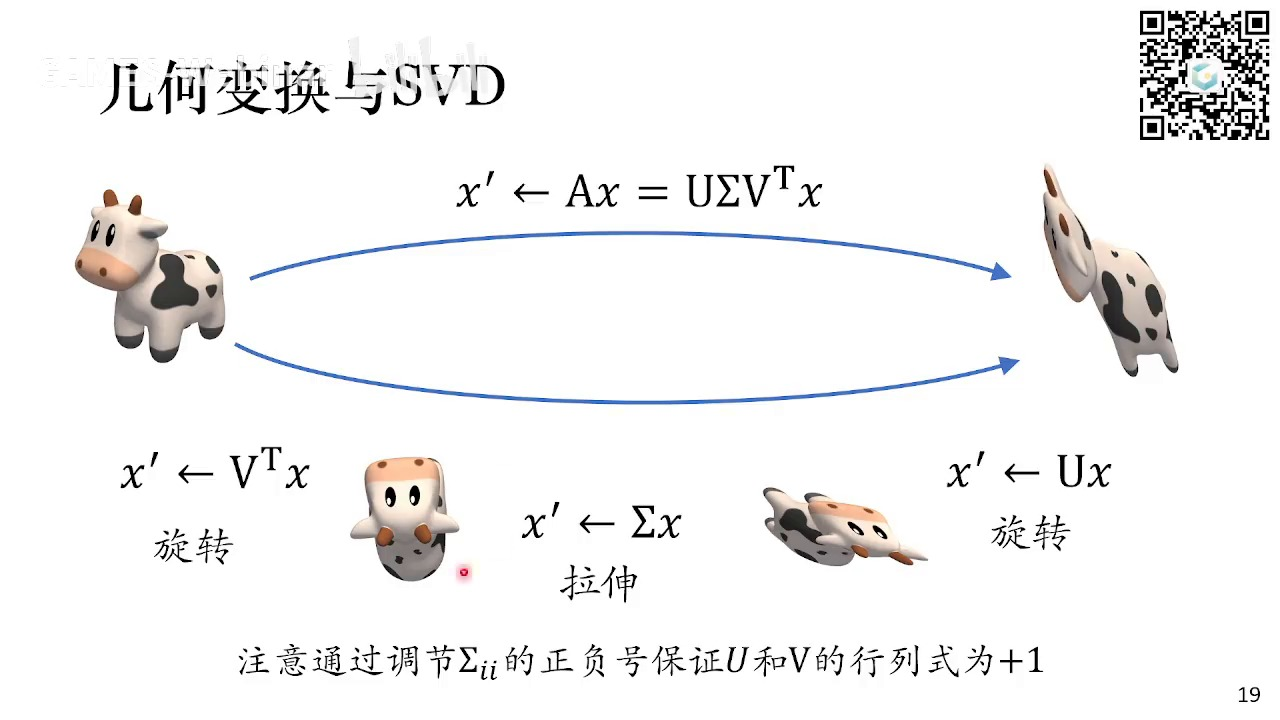
\includegraphics[width=0.92\textwidth]{figures/fig_16_geo_svd.jpg}
\caption{SVD 的几何意义：旋转 $\mathrm V^{\mathsf T}$、拉伸 $\Sigma$、旋转 $\mathrm U$\vtag}
\end{figure}
\srcnote{00:52:30--00:52:45}
\end{minipage}


\subsection{极分解}

\textbf{极分解}（polar decomposition）：对任意实方阵 $\mathrm A$，存在唯一的正交矩阵 $\mathrm R$ 和半正定矩阵 $\mathrm S$，使得 $\mathrm A=\mathrm R\mathrm S$（$\mathrm A$ 可逆时唯一）。从 SVD 的角度看，它的推导非常直接，只要在中间插入 $\mathrm V^{\mathsf T}\mathrm V$ 或 $\mathrm U^{\mathsf T}\mathrm U$：
\[
\mathrm A=\mathrm U\Sigma\mathrm V^{\mathsf T}=(\mathrm U\mathrm V^{\mathsf T})(\mathrm V\Sigma\mathrm V^{\mathsf T})=(\mathrm U\Sigma\mathrm U^{\mathsf T})(\mathrm U\mathrm V^{\mathsf T}).
\]
$\mathrm U\mathrm V^{\mathsf T}$ 是正交矩阵，对应旋转；$\mathrm V\Sigma\mathrm V^{\mathsf T}$ 和 $\mathrm U\Sigma\mathrm U^{\mathsf T}$ 是半正定矩阵，对应拉伸：先转一个角度、拉伸一下、再转回来。所以既可以先拉伸后旋转，也可以先旋转后拉伸；两种写法中旋转都是 $\mathrm U\mathrm V^{\mathsf T}$，但拉伸矩阵不一样。

\noindent\begin{minipage}{\textwidth}
\begin{figure}[H]
\centering
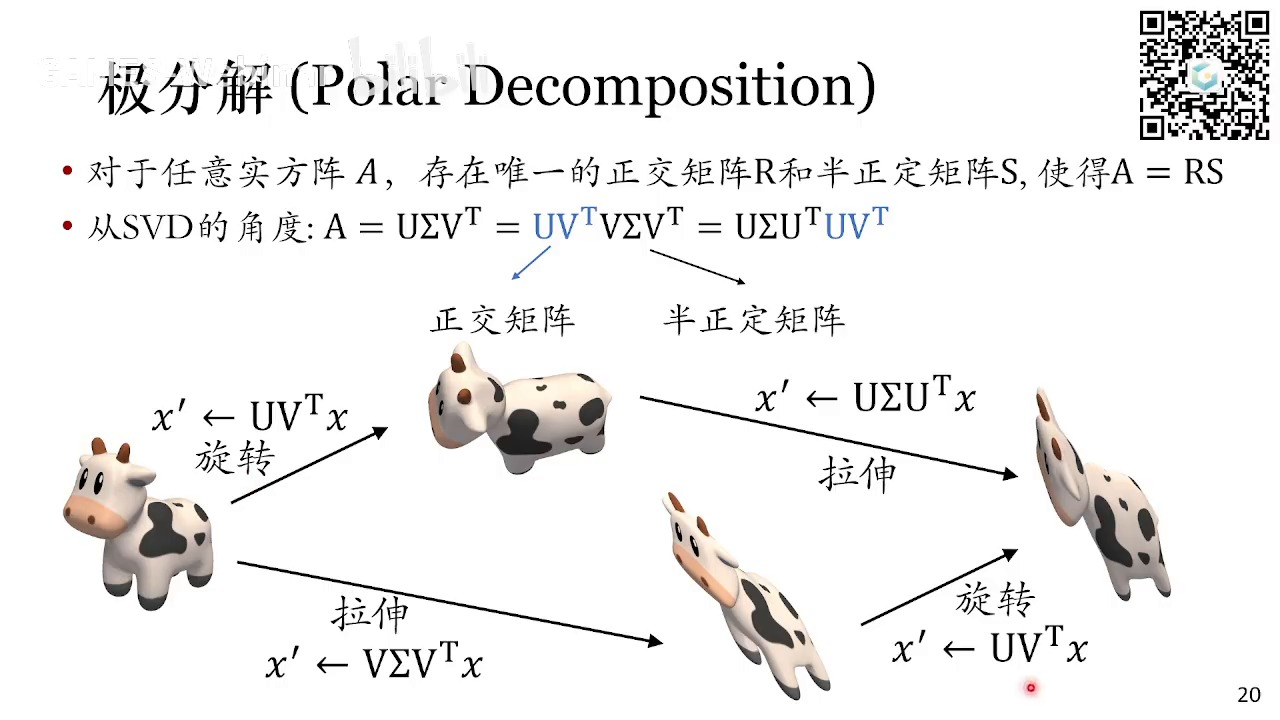
\includegraphics[width=0.92\textwidth]{figures/fig_17_polar.jpg}
\caption{极分解：$\mathrm A=\mathrm R\mathrm S$，先拉伸后旋转或先旋转后拉伸\vtag}
\end{figure}
\srcnote{00:56:00--00:56:15}
\end{minipage}


\begin{knowledgebox}{极分解在模拟中的用途}
讲义作者补充：在弹性体和连续介质模拟中，形变梯度 $\mathrm F$ 的极分解 $\mathrm F=\mathrm R\mathrm S$ 把“刚体旋转”与“真正的拉伸”分开。许多本构模型（如 co-rotational 模型）只对 $\mathrm S$ 计算能量，从而让能量对刚体旋转保持不变。下面的形状匹配，就是从一组点的对应关系中提取这个旋转。
\end{knowledgebox}

\section{应用一：形状匹配}

\subsection{问题与平移}

对于形变 $\mathbf q\to\mathbf p$，如何得到最接近它的刚性变换？也就是求
\[
\mathrm R,\mathbf t=\operatorname*{argmin}\sum_i\|\mathbf p_i-(\mathrm R\mathbf q_i+\mathbf t)\|^2 .
\]
讲者说，这个算法解决的就是这样的问题：给定任意的形变，找一个刚性变换，让模型尽可能接近形变后的结果。这个任意的形变里面可能有旋转，可能有拉伸，甚至可能有非线性的变换；我们要做的是只用一个旋转加一个平移去变换点 $\mathbf q$，让它尽可能接近最后的结果 $\mathbf p$。这个问题和奇异值分解有着紧密的联系，在物理模拟中的“形状匹配”方法、刚体配准和点云对齐中都会用到。

\noindent\begin{minipage}{\textwidth}
\begin{figure}[H]
\centering
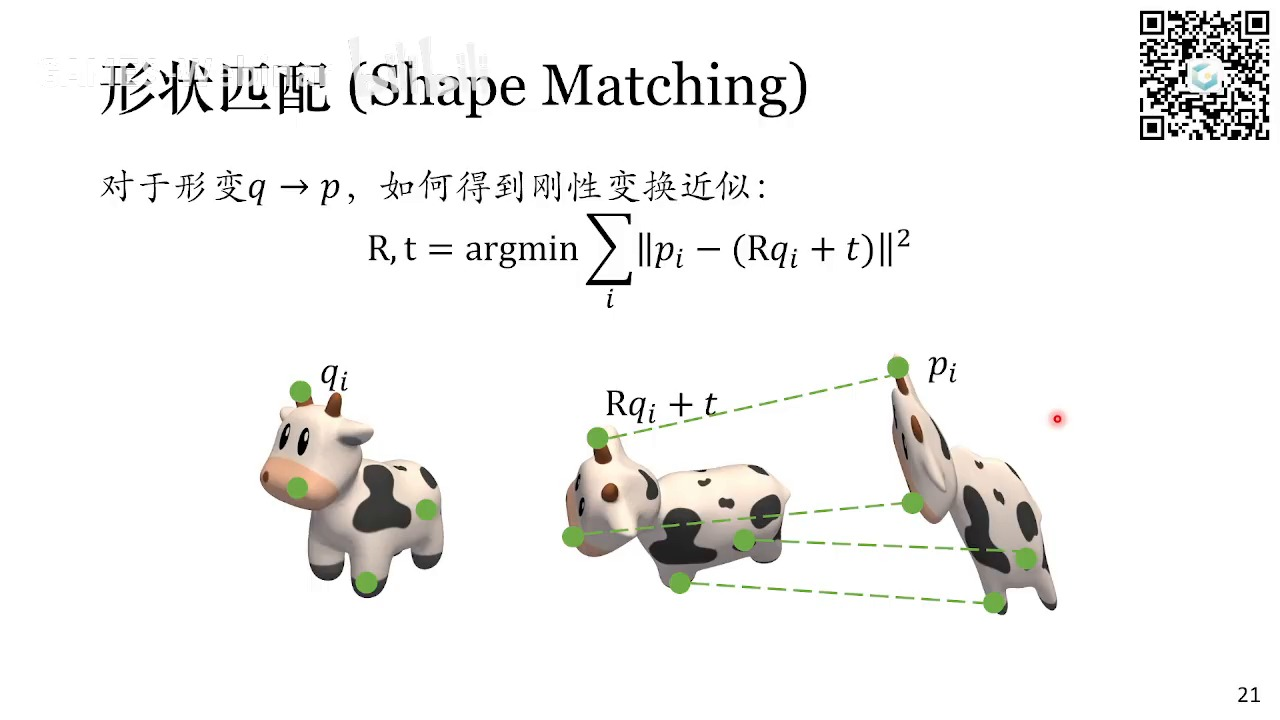
\includegraphics[width=0.92\textwidth]{figures/fig_18_shape_match_def.jpg}
\caption{形状匹配：为形变 $\mathbf q\to\mathbf p$ 寻找最接近的刚性变换 $(\mathrm R,\mathbf t)$\vtag}
\end{figure}
\srcnote{00:57:45--00:58:00}
\end{minipage}


先在 $\mathrm R$ 给定时只考虑 $\mathbf t$。对目标函数求导：
\[
\frac{\partial}{\partial\mathbf t}\sum_i\|\mathbf p_i-(\mathrm R\mathbf q_i+\mathbf t)\|^2=2\sum_i(\mathrm R\mathbf q_i+\mathbf t-\mathbf p_i)=0
\;\Longrightarrow\;
n\mathbf t=\sum_i\mathbf p_i-\mathrm R\sum_i\mathbf q_i .
\]
记形变前后的质心为 $\mathbf q_c=\frac1n\sum\mathbf q_i$，$\mathbf p_c=\frac1n\sum\mathbf p_i$，则 $\mathbf t=\mathbf p_c-\mathrm R\mathbf q_c$。

\noindent\begin{minipage}{\textwidth}
\begin{figure}[H]
\centering
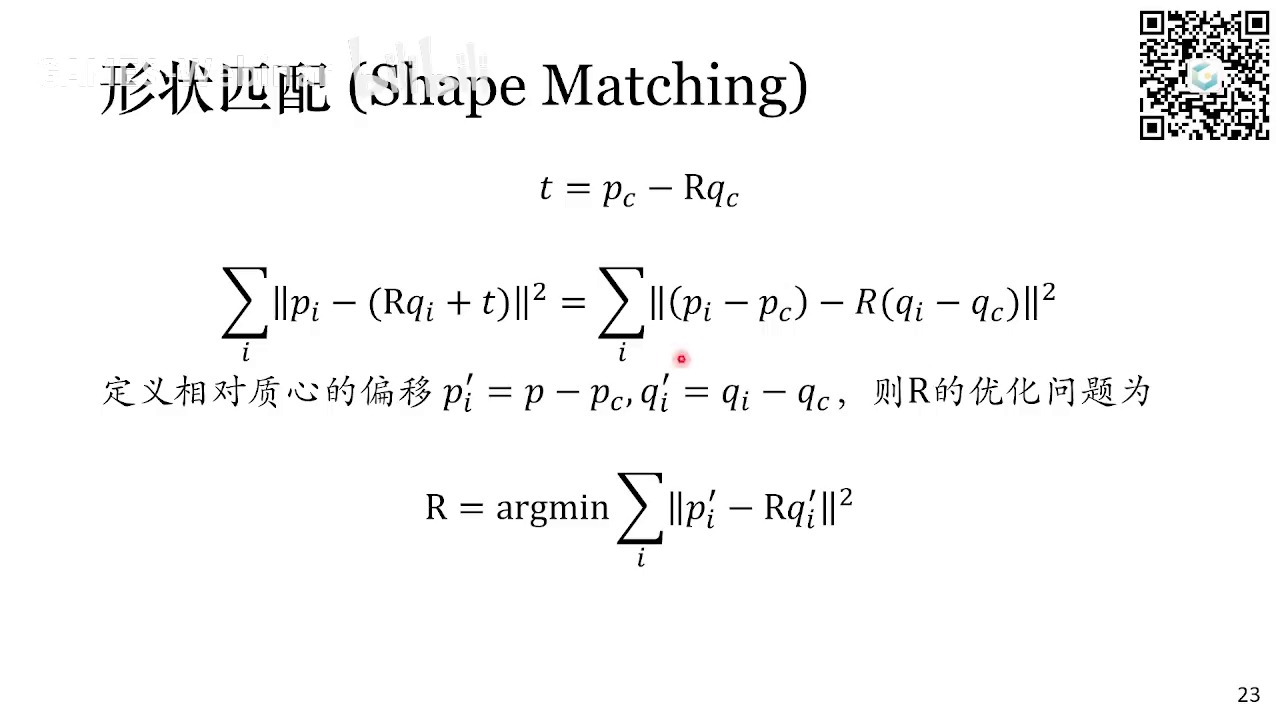
\includegraphics[width=0.92\textwidth]{figures/fig_19_shape_t.jpg}
\caption{固定 $\mathrm R$ 求 $\mathbf t$：$\mathbf t=\mathbf p_c-\mathrm R\mathbf q_c$\vtag}
\end{figure}
\srcnote{00:59:45--01:00:00}
\end{minipage}


\subsection{化为迹的最大化}

把 $\mathbf t$ 代回，定义相对质心的偏移 $\mathbf p'_i=\mathbf p_i-\mathbf p_c$，$\mathbf q'_i=\mathbf q_i-\mathbf q_c$，旋转的优化问题变为
\[
\mathrm R=\operatorname*{argmin}\sum_i\|\mathbf p'_i-\mathrm R\mathbf q'_i\|^2 .
\]
展开平方：$\mathbf p'^{\mathsf T}_i\mathbf p'_i$ 与 $\mathrm R$ 无关；由于 $\mathrm R^{\mathsf T}\mathrm R=\mathrm I$，$\mathbf q'^{\mathsf T}_i\mathrm R^{\mathsf T}\mathrm R\mathbf q'_i$ 也与 $\mathrm R$ 无关；剩下的两项交叉项相等。所以最小化等价于最大化交叉项。每一项是标量，可以写成迹并循环置换：
\[
\sum_i\mathbf p'^{\mathsf T}_i\mathrm R\mathbf q'_i=\operatorname{Tr}\Big(\sum_i\mathbf p'^{\mathsf T}_i\mathrm R\mathbf q'_i\Big)=\operatorname{Tr}\Big(\mathrm R\sum_i\mathbf q'_i\mathbf p'^{\mathsf T}_i\Big),\qquad
\max_{\mathrm R}\operatorname{Tr}(\mathrm R\mathrm H),\quad \mathrm H=\sum_i\mathbf q'_i\mathbf p'^{\mathsf T}_i .
\]
求和里已经和 $\mathrm R$ 无关，$\mathrm H$ 是一个常数矩阵。

\noindent\begin{minipage}{\textwidth}
\begin{figure}[H]
\centering
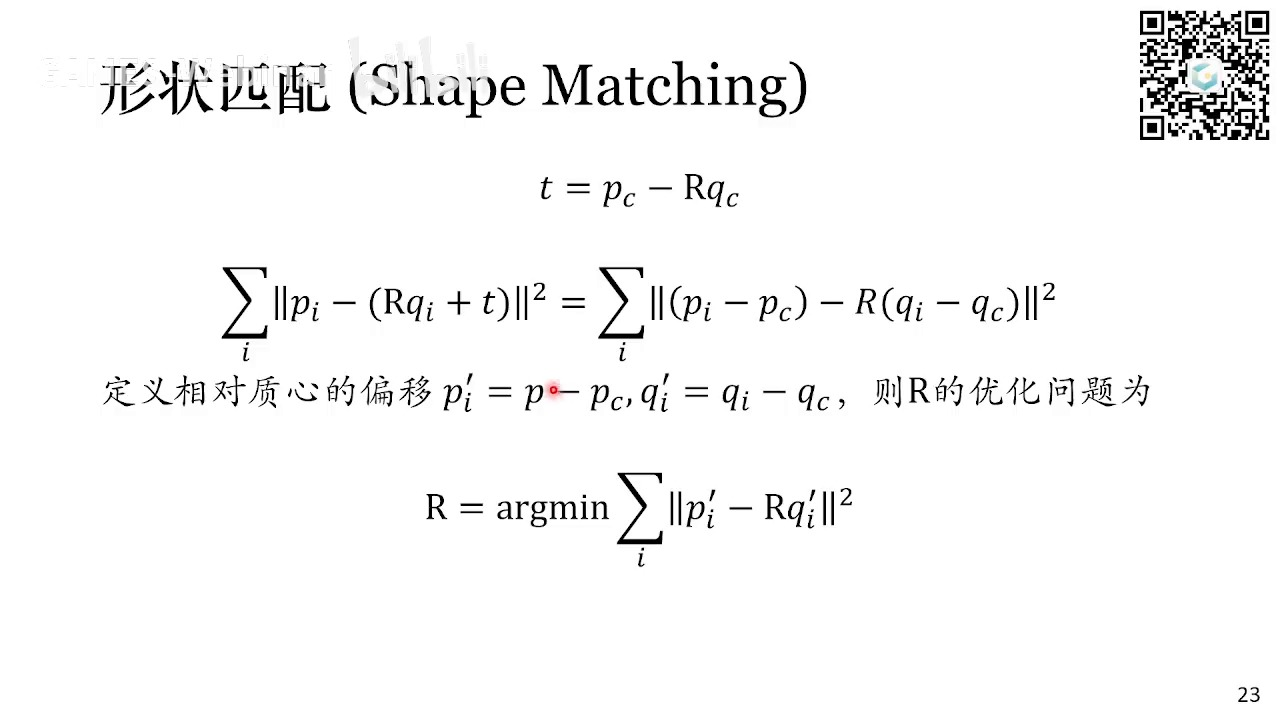
\includegraphics[width=0.92\textwidth]{figures/fig_20_shape_r.jpg}
\caption{代入平移后，旋转的优化只依赖相对质心的偏移\vtag}
\end{figure}
\srcnote{01:00:00--01:00:15}
\end{minipage}


\noindent\begin{minipage}{\textwidth}
\begin{figure}[H]
\centering
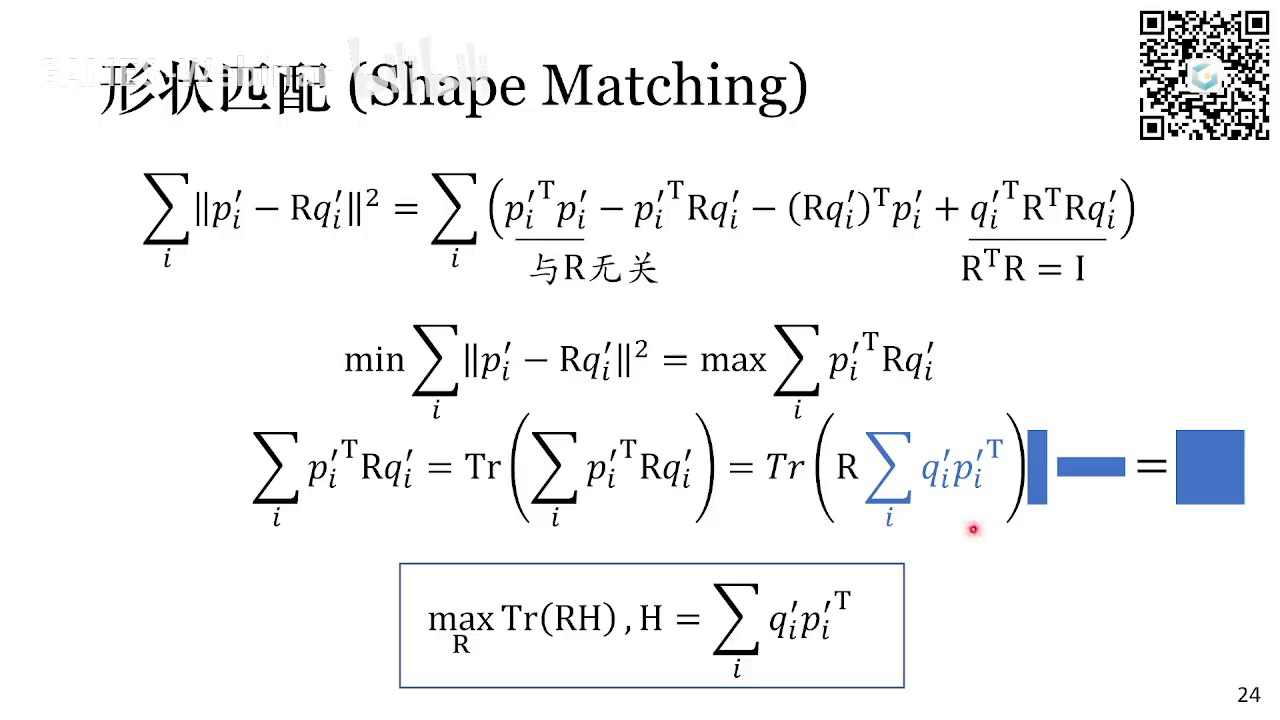
\includegraphics[width=0.92\textwidth]{figures/fig_21_shape_trace.jpg}
\caption{最小化残差等价于最大化 $\operatorname{Tr}(\mathrm R\mathrm H)$\vtag}
\end{figure}
\srcnote{01:03:00--01:03:15}
\end{minipage}


\subsection{一个关于迹的不等式}

\textbf{定理}：对于对称正定矩阵 $\mathrm M$ 和正交矩阵 $\mathrm B$，一定有 $\operatorname{Tr}\mathrm M\ge\operatorname{Tr}(\mathrm B\mathrm M)$。

证明：对 $\mathrm M$ 做特征值分解 $\mathrm Q\Lambda\mathrm Q^{\mathsf T}$，令 $\mathrm S=\mathrm Q\Lambda^{1/2}\mathrm Q^{\mathsf T}$，则 $\mathrm S^2=\mathrm S^{\mathsf T}\mathrm S=\mathrm M$。于是
\[
\operatorname{Tr}(\mathrm B\mathrm M)=\operatorname{Tr}(\mathrm B\mathrm S^2)=\operatorname{Tr}(\mathrm S\mathrm B\mathrm S)=\operatorname{Tr}(\mathrm S^{\mathsf T}\mathrm B\mathrm S).
\]
记 $\mathbf s_i$ 为 $\mathrm S$ 的第 $i$ 列，对角项 $(\mathrm S^{\mathsf T}\mathrm S)_{ii}=\mathbf s_i^{\mathsf T}\mathbf s_i$，$(\mathrm S^{\mathsf T}\mathrm B\mathrm S)_{ii}=\mathbf s_i^{\mathsf T}\mathrm B\mathbf s_i$。正交矩阵不改变 $\mathbf s_i$ 的长度，由柯西—施瓦茨不等式 $\mathbf s_i^{\mathsf T}\mathrm B\mathbf s_i\le\|\mathbf s_i\|\,\|\mathrm B\mathbf s_i\|=\mathbf s_i^{\mathsf T}\mathbf s_i$，从而
\[
\operatorname{Tr}(\mathrm B\mathrm M)=\sum_i\mathbf s_i^{\mathsf T}\mathrm B\mathbf s_i\le\sum_i\mathbf s_i^{\mathsf T}\mathbf s_i=\operatorname{Tr}\mathrm M .
\]
讲者说这部分证明稍微复杂，不理解也没关系，可以直接记结论。

\noindent\begin{minipage}{\textwidth}
\begin{figure}[H]
\centering
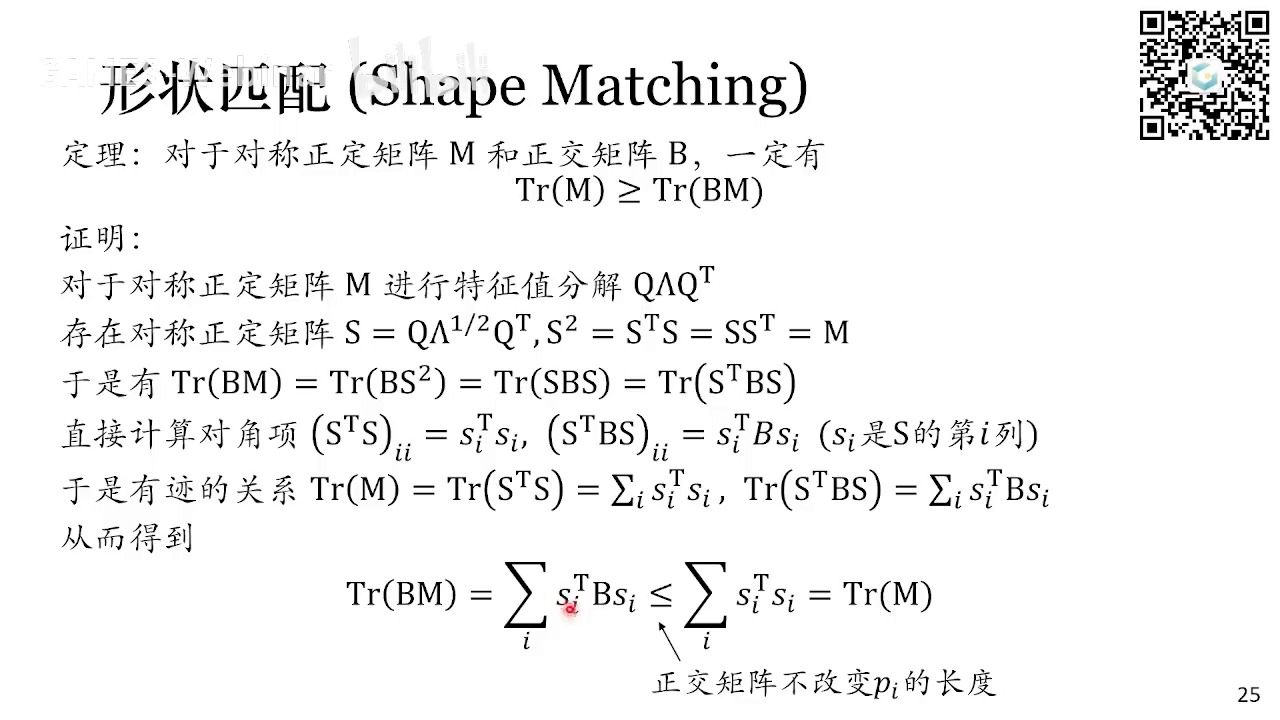
\includegraphics[width=0.92\textwidth]{figures/fig_22_trace_thm.jpg}
\caption{定理：对称正定 $\mathrm M$ 与正交 $\mathrm B$ 满足 $\operatorname{Tr}\mathrm M\ge\operatorname{Tr}(\mathrm B\mathrm M)$\vtag}
\end{figure}
\srcnote{01:06:00--01:06:15}
\end{minipage}


\subsection{用 SVD 求最优旋转}

如果某个 $\mathrm R^*$ 能使 $\mathrm R^*\mathrm H$ 为对称正定矩阵，那么对任意旋转 $\mathrm R$，在中间插入 $\mathrm R^{*\mathsf T}\mathrm R^*$：
\[
\operatorname{Tr}(\mathrm R\mathrm H)=\operatorname{Tr}\big((\mathrm R\mathrm R^{*\mathsf T})(\mathrm R^*\mathrm H)\big)\le\operatorname{Tr}(\mathrm R^*\mathrm H),
\]
前一个因子是正交矩阵 $\mathrm B$，后一个是对称矩阵 $\mathrm M$，由定理即得。讲者解释了为什么要在中间插入 $\mathrm R^{*\mathsf T}\mathrm R^*$：插入以后，前面两个旋转结合成一个正交矩阵，后面结合成一个对称矩阵，正好套用刚才的定理。所以问题转化为：找一个旋转，使它乘以 $\mathrm H$ 后变成对称正定矩阵，这个旋转就是最优解。$\mathrm R\mathrm H$ 何时对称正定？对 $\mathrm H$ 做 SVD，$\mathrm H=\mathrm U\Sigma\mathrm V^{\mathsf T}$，取 $\mathrm R=\mathrm V\mathrm U^{\mathsf T}$，则 $\mathrm R\mathrm H=\mathrm V\Sigma\mathrm V^{\mathsf T}$，正是对称半正定的。因为 $\Sigma$ 的每一项都非负，而 $\mathrm V$ 与 $\mathrm V^{\mathsf T}$ 分列两侧，形成的是一个对称的二次型结构。

如果 $\det(\mathrm V\mathrm U^{\mathsf T})=-1$，$\mathrm V\mathrm U^{\mathsf T}$ 是镜像而不是旋转，需要在中间乘一个修正矩阵：
\[
\mathrm R=\mathrm V\begin{pmatrix}1&&\\&1&\\&&\det(\mathrm V\mathrm U^{\mathsf T})\end{pmatrix}\mathrm U^{\mathsf T}.
\]
详细推导可参考 Olga Sorkine-Hornung 的笔记（igl.ethz.ch/projects/ARAP/svd\_rot.pdf）。

\noindent\begin{minipage}{\textwidth}
\begin{figure}[H]
\centering
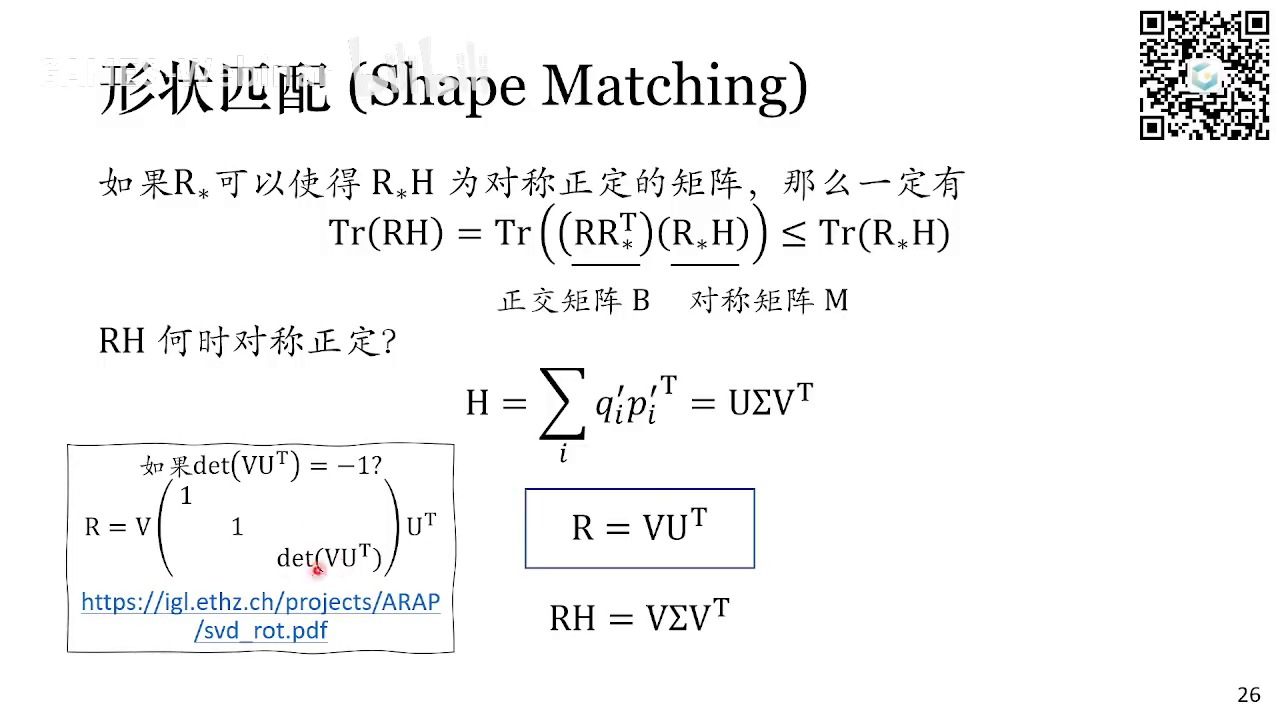
\includegraphics[width=0.92\textwidth]{figures/fig_23_shape_svd.jpg}
\caption{由 $\mathrm H=\mathrm U\Sigma\mathrm V^{\mathsf T}$ 取 $\mathrm R=\mathrm V\mathrm U^{\mathsf T}$，并处理 $\det=-1$ 的情况\vtag}
\end{figure}
\srcnote{01:09:15--01:09:30}
\end{minipage}


\begin{practicebox}{形状匹配算法流程}
\begin{enumerate}
\item 计算相对质心的偏移：$\mathbf q'_i=\mathbf q_i-\mathbf q_c$，$\mathbf p'_i=\mathbf p_i-\mathbf p_c$。
\item 构造 $\mathrm H=\sum_i\mathbf q'_i\mathbf p'^{\mathsf T}_i$，做 SVD：$\mathrm H=\mathrm U\Sigma\mathrm V^{\mathsf T}$。
\item 得到最优旋转 $\mathrm R=\mathrm V\mathrm U^{\mathsf T}$；若行列式为 $-1$，按上式修正。
\item 得到平移 $\mathbf t=\mathbf p_c-\mathrm R\mathbf q_c$。
\end{enumerate}
有了 $\mathrm R$ 和 $\mathbf t$，就可以把两个形状或两张图片对齐到一起。
讲者说推导可以不记，但这个算法流程非常经典，值得记下来。读者可以随机生成一组点，施加已知的旋转、平移和少量噪声，验证算法能否恢复它们。
\end{practicebox}

\noindent\begin{minipage}{\textwidth}
\begin{figure}[H]
\centering
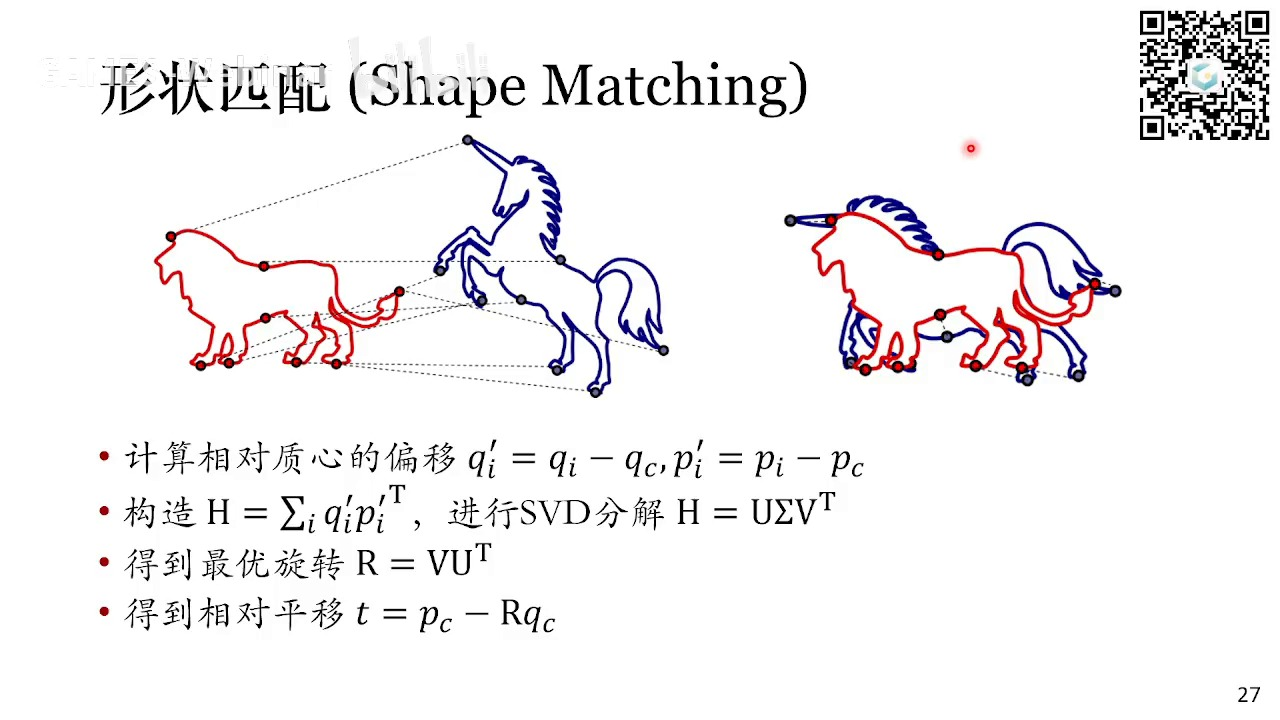
\includegraphics[width=0.92\textwidth]{figures/fig_24_shape_algo.jpg}
\caption{形状匹配的算法流程与示例\vtag}
\end{figure}
\srcnote{01:11:15--01:11:30}
\end{minipage}


\section{应用二：图像压缩与 LoRA}

\subsection{低秩近似}

分辨率为 $m\times n$ 的图像可以看成一个大型稠密矩阵 $\mathrm A\in\mathbb R^{m\times n}$。把 SVD 换一种写法，按列展开：
\[
\mathrm A=\mathrm U\Sigma\mathrm V^{\mathsf T}=\sum_i\sigma_i\mathbf u_i\mathbf v_i^{\mathsf T},
\]
每一项 $\sigma_i\mathbf u_i\mathbf v_i^{\mathsf T}$ 都是秩为 1 的矩阵。具体地说，第 $i$ 项是把 $\Sigma$ 的第 $i$ 个对角元拿出来，乘以 $\mathrm U$ 的第 $i$ 列和 $\mathrm V^{\mathsf T}$ 的第 $i$ 行；一列乘一行得到的矩阵，秩一定是 1。由于奇异值按从大到小排列，这个求和天然是按“重要性”排好序的。压缩时把求和截断，只保留前面几项。

\noindent\begin{minipage}{\textwidth}
\begin{figure}[H]
\centering
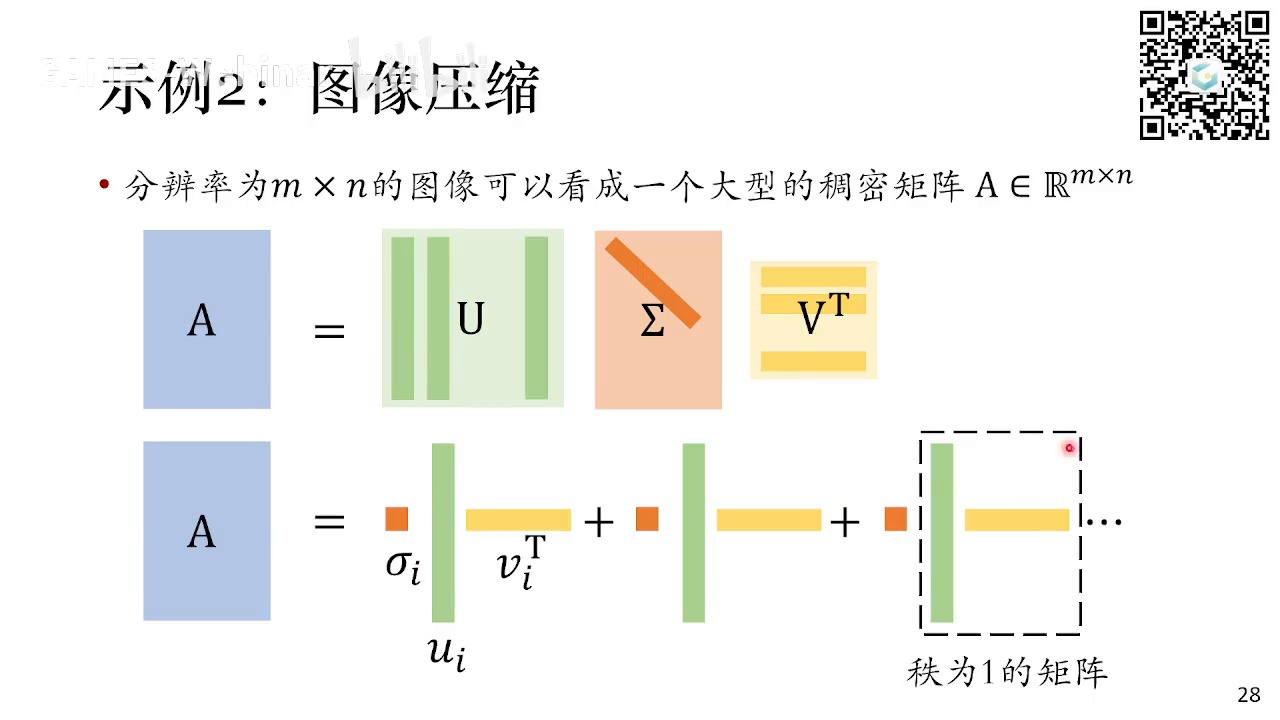
\includegraphics[width=0.92\textwidth]{figures/fig_25_image_matrix.jpg}
\caption{图像压缩：把图像矩阵写成秩 1 矩阵之和并截断\vtag}
\end{figure}
\srcnote{01:13:15--01:13:30}
\end{minipage}


为什么可以截断？看一张 $512\times512$ 图片的奇异值分布：前面几个最大的奇异值占了整张图片很重要的比重，后面大量的小奇异值只贡献细节。它们前面的系数很小，在求和中就不那么重要了。所以要压缩图像，只需要在奇异值序列的某个位置截断，对这张图来说，大概在几十的位置截断就足够。

\noindent\begin{minipage}{\textwidth}
\begin{figure}[H]
\centering
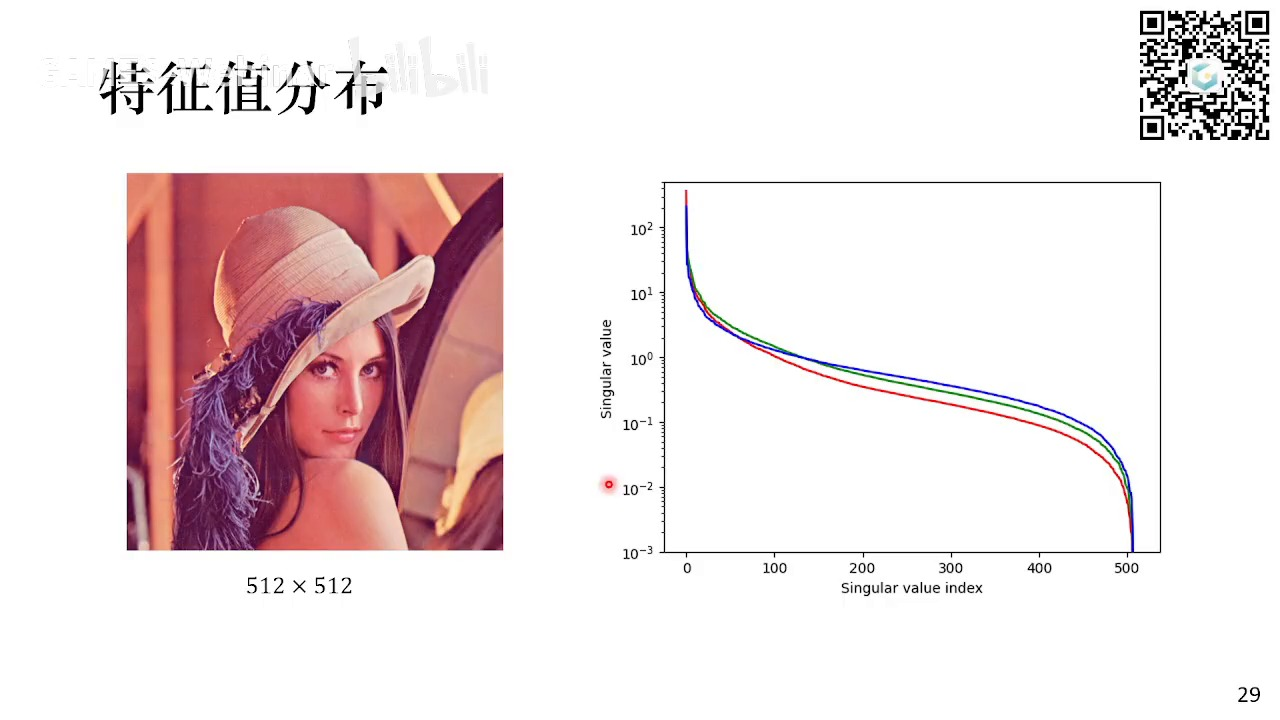
\includegraphics[width=0.92\textwidth]{figures/fig_26_sv_distribution.jpg}
\caption{$512\times512$ 图片的奇异值分布：少数大奇异值占主导\vtag}
\end{figure}
\srcnote{01:14:45--01:15:00}
\end{minipage}


只保留 1 个奇异值时，图像只剩一个秩 1 矩阵，满是横竖条纹，基本看不出原来的内容，压缩过度了；保留到 4 个时大概能看出有人形；保留 16 个时已经能辨认；此时所用的内存只占原图的 3.15\%，图片却已经大致可以辨认；保留 64 个时与原图相当接近。讲者还指出，在图片中原本光滑的区域，截断后反而去掉了很多噪点，因为噪声主要存在于被丢掉的小奇异值里。

\noindent\begin{minipage}{\textwidth}
\begin{figure}[H]
\centering
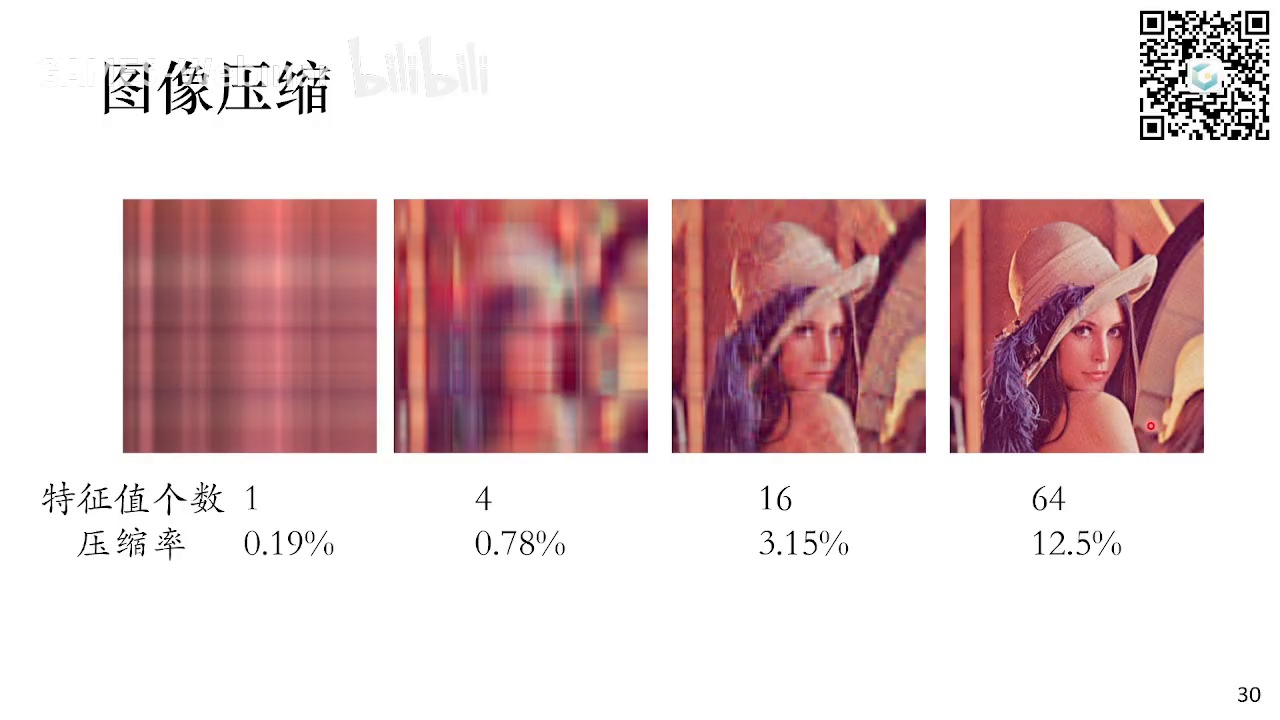
\includegraphics[width=0.92\textwidth]{figures/fig_27_image_compress.jpg}
\caption{保留 1、4、16、64 个奇异值的压缩效果（课件标注压缩率 0.19\%、0.78\%、3.15\%、12.5\%）\vtag}
\end{figure}
\srcnote{01:17:00--01:17:15}
\end{minipage}


\begin{warningbox}{压缩率怎么算}
讲者解释保留 16 项时的压缩率：原图要存 $512\times512$ 个像素，而每个秩 1 矩阵只需存两个长度为 512 的向量（再加一个奇异值）。讲义作者提醒：按这个口径，保留 $k$ 项的存储比为 $k(2\cdot512+1)/512^2$，$k=16$ 时约为 6.3\%；课件中的 0.19\%、0.78\%、3.15\%、12.5\% 实际上是 $k/512$，相当于只计了一个向量。数量级的结论不变：远小于原图。
\end{warningbox}

\subsection{LoRA}

同样的思想被用在大模型微调中。讲者说，这种低秩压缩的思想最近在大语言模型领域非常有用，其中一项很重要的技术就是 LoRA。对于大语言模型，参数量动辄以十亿计，全部重新训练几乎不可能，微调成为常态。LoRA（low-rank adaptation of large language models）的出发点是：大模型的权重矩阵 $\mathrm W$ 非常大，每次前向和反向传播都要处理它，训练成本很高。微调时其实只需要改增量，LoRA 就像 SVD 压缩那样，用两个秩为 $r$（$r$ 很小）的矩阵相乘来表示增量：
\[
\mathrm W'=\mathrm W+\Delta\mathrm W,\qquad \Delta\mathrm W=\mathrm B\mathrm A,\quad \mathrm B\in\mathbb R^{d\times r},\ \mathrm A\in\mathbb R^{r\times k} .
\]
只训练这两个小矩阵，参数量大幅减少，训练的经济性很高；又因为权重中的信息本来就可以用低秩形式压缩，信息不会丢失太多。讲者强调这只是 LoRA 的基本思想，它还有许多技术细节。

\begin{practicebox}{动手做图像压缩}
找一张灰度图片读成矩阵，用任意线性代数库做 SVD，画出奇异值随序号下降的曲线；再分别保留前 1、4、16、64 个奇异值重建图像，观察条纹、轮廓和细节依次出现的过程，并按 $k(m+n+1)/(mn)$ 计算每种情况的存储比。也可以对彩色图片的三个通道分别做，比较哪个通道需要的奇异值更多。
\end{practicebox}

\noindent\begin{minipage}{\textwidth}
\begin{figure}[H]
\centering
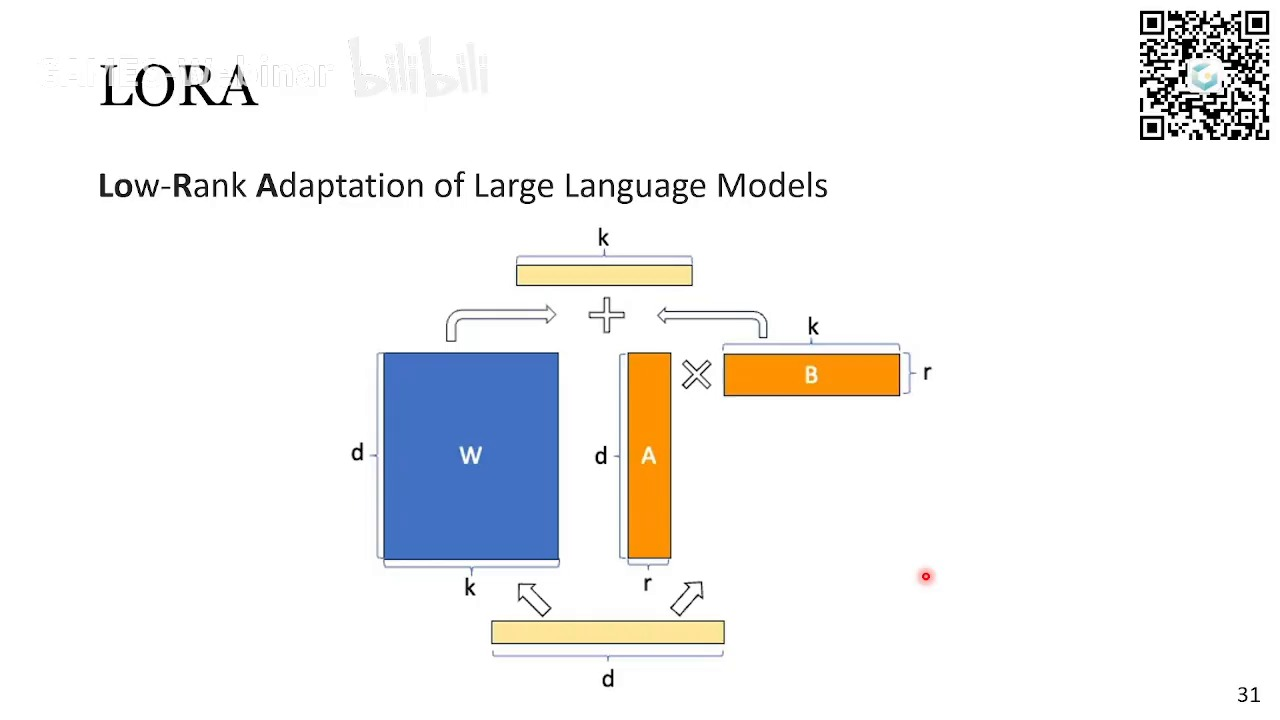
\includegraphics[width=0.92\textwidth]{figures/fig_28_lora.jpg}
\caption{LoRA：用两个低秩矩阵表示权重增量\vtag}
\end{figure}
\srcnote{01:19:30--01:19:45}
\end{minipage}


\section{应用三：SVD 的求导与效率}

\subsection{为什么需要对 SVD 求导}

SVD 是可微运算。在弹性体模拟中，能量常写成形变梯度奇异值的函数，需要 $\partial\Sigma/\partial\mathrm A$ 和极分解中 $\partial\mathrm R/\partial\mathrm A$；把 SVD 作为神经网络的一个模块时，反向传播需要已知 $\delta\mathrm A$ 求 $\delta\Sigma$ 和 $\delta\mathrm R$。换句话说，只要 SVD 出现在计算图中间，无论是物理模拟里用牛顿法求能量的梯度和海森矩阵，还是神经网络里做端到端训练，都绕不开“分解结果对原矩阵的导数”这个问题。讲者在这里只给出奇异值的情形作为示例，旋转部分的导数推导思路相同，但更繁琐。

\noindent\begin{minipage}{\textwidth}
\begin{figure}[H]
\centering
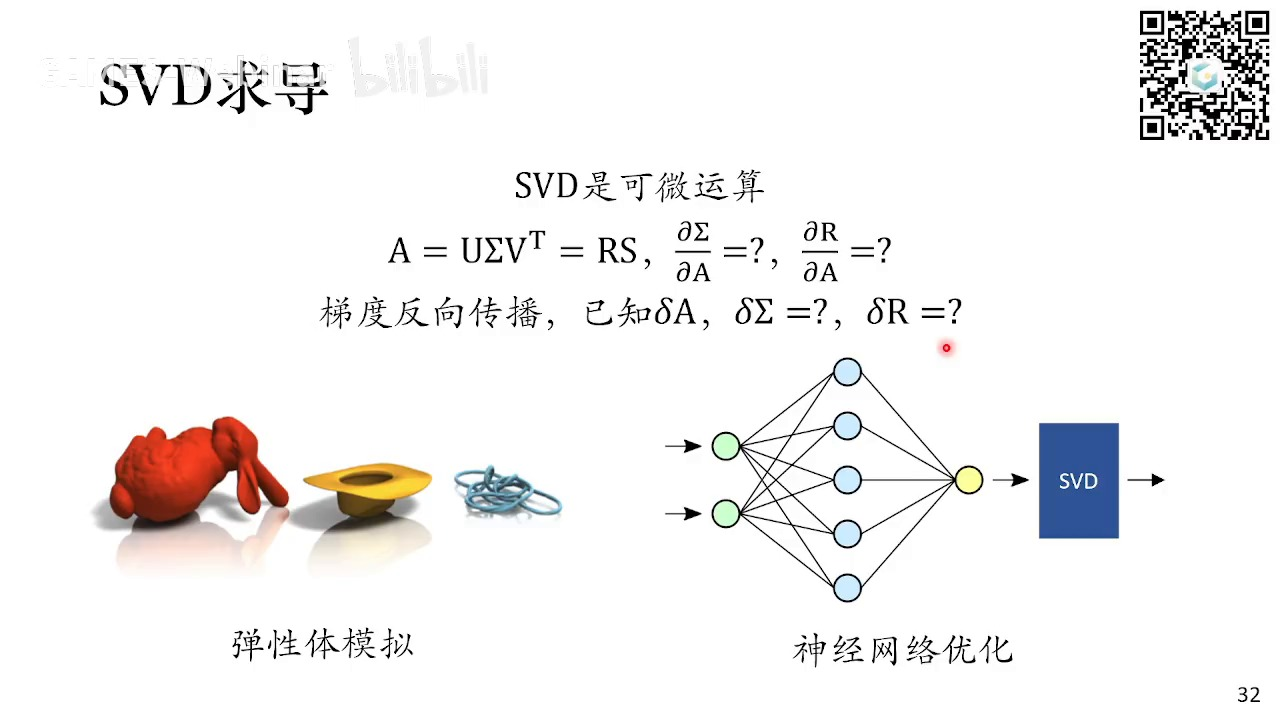
\includegraphics[width=0.92\textwidth]{figures/fig_29_svd_grad.jpg}
\caption{SVD 求导的需求：弹性体模拟与神经网络优化\vtag}
\end{figure}
\srcnote{01:20:30--01:20:45}
\end{minipage}


\subsection{奇异值的导数}

设 $\mathrm F=\mathrm U\Sigma\mathrm V^{\mathsf T}$，对其求微分：
\[
\delta\mathrm F=\delta\mathrm U\,\Sigma\mathrm V^{\mathsf T}+\mathrm U\,\delta\Sigma\,\mathrm V^{\mathsf T}+\mathrm U\Sigma\,\delta\mathrm V^{\mathsf T}
\;\Longrightarrow\;
\delta\Sigma=\mathrm U^{\mathsf T}\delta\mathrm F\,\mathrm V-\mathrm U^{\mathsf T}\delta\mathrm U\,\Sigma-\Sigma\,\delta\mathrm V^{\mathsf T}\mathrm V .
\]
$\mathrm U^{\mathsf T}\delta\mathrm U$ 和 $\mathrm V^{\mathsf T}\delta\mathrm V$ 都是反对称矩阵，这在上一讲旋转求导时已经见过：对 $\mathrm U^{\mathsf T}\mathrm U=\mathrm I$ 求微分，$\delta\mathrm U^{\mathsf T}\mathrm U+\mathrm U^{\mathsf T}\delta\mathrm U=0$。反对称矩阵的对角线为零，乘以对角矩阵 $\Sigma$ 后对角线仍为零，所以只取对角部分：
\[
\delta\Sigma=\operatorname{Diag}\big(\mathrm U^{\mathsf T}\delta\mathrm F\,\mathrm V\big),\qquad\text{即}\quad \frac{\partial\sigma_i}{\partial\mathrm F}=\mathbf u_i\mathbf v_i^{\mathsf T}.
\]

\noindent\begin{minipage}{\textwidth}
\begin{figure}[H]
\centering
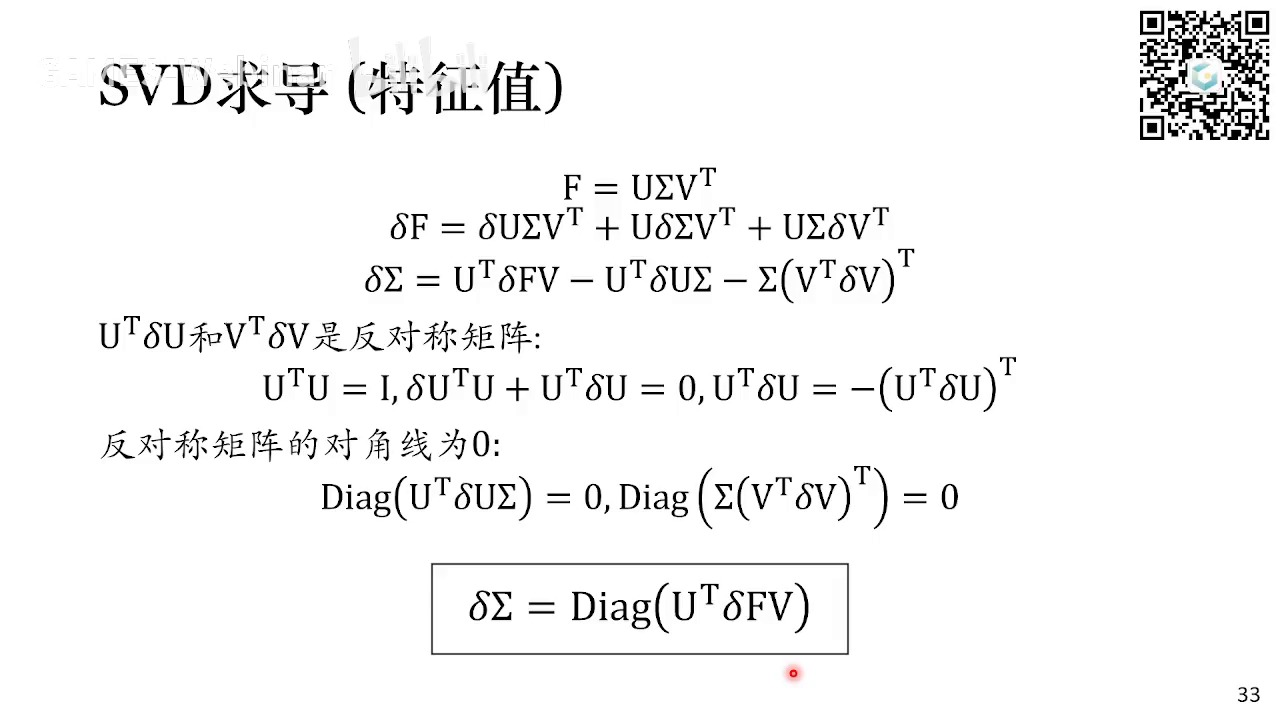
\includegraphics[width=0.92\textwidth]{figures/fig_30_svd_grad_sigma.jpg}
\caption{奇异值的导数：利用 $\mathrm U^{\mathsf T}\delta\mathrm U$ 反对称，$\delta\Sigma=\operatorname{Diag}(\mathrm U^{\mathsf T}\delta\mathrm F\mathrm V)$\vtag}
\end{figure}
\srcnote{01:23:15--01:23:30}
\end{minipage}


\begin{warningbox}{SVD 很耗时}
一般来说，SVD 是比较耗时的算法。好在现有实现比较齐全：有专门快速计算 $3\times3$ 矩阵 SVD 的算法，大规模稠密或稀疏线性代数库基本都提供优化过的接口，大部分时候调包即可。但在每帧、每个单元都要调用的模拟代码里，一定要注意 SVD 的开销。此外，奇异值相等时 $\mathrm U,\mathrm V$ 的导数会出现除以 $\sigma_i^2-\sigma_j^2$ 的项，需要特殊处理。
\end{warningbox}

\noindent\begin{minipage}{\textwidth}
\begin{figure}[H]
\centering
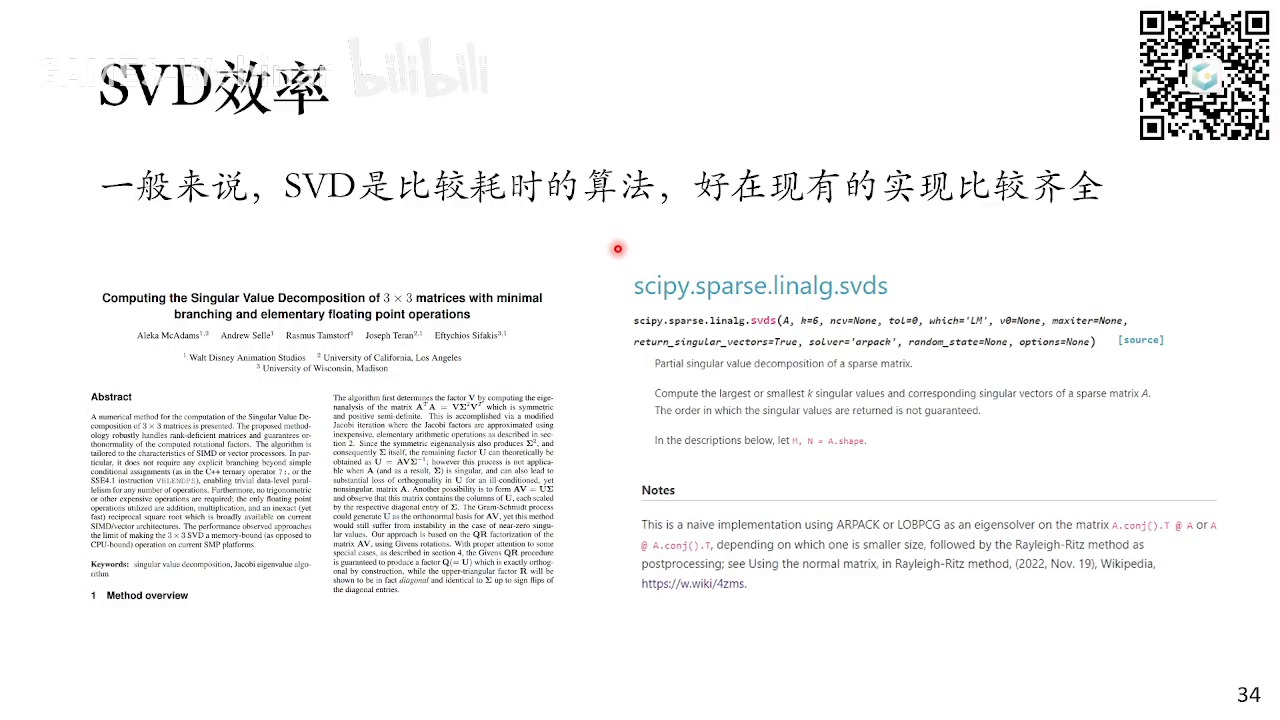
\includegraphics[width=0.92\textwidth]{figures/fig_31_svd_efficiency.jpg}
\caption{SVD 的效率：耗时，但现有实现齐全\vtag}
\end{figure}
\srcnote{01:24:30--01:24:45}
\end{minipage}


讲者在这里回答了弹幕的问题。有同学问张量分解是否与 SVD 类似：张量分解可以看作 SVD 向高阶张量的推广，但已超出本课范围。他还推荐了 Gilbert Strang 在 MIT 的线性代数课程与讲义，认为它是公认最好的线性代数课；并说明 GAMES001 的定位是：后续课程中遇到哪块数学不清楚，可以回来查，而不是必须先学完。

\section{主成分分析}

\subsection{降维表达}

PCA 的经典例子是 Eigenfaces。它要解决的问题是降维：有一堆二维数据点，能否找一个方向，把它们投影到一维，同时尽量保留数据的信息？关键在于如何选择投影方向。比如在图中找一条倾斜的直线，把所有点投影上去，点在直线上的分布就是一维的表达。不同的直线保留的信息不同：讲者对比了两种方向，若选的方向使投影后的点分布得非常集中，原来点与点之间的差别就丢掉了；若选的是图中绿色的方向，投影后的点分布得比较分散，这个方向显然更能代表数据集。下面从低阶到高阶一步步来。

\noindent\begin{minipage}{\textwidth}
\begin{figure}[H]
\centering
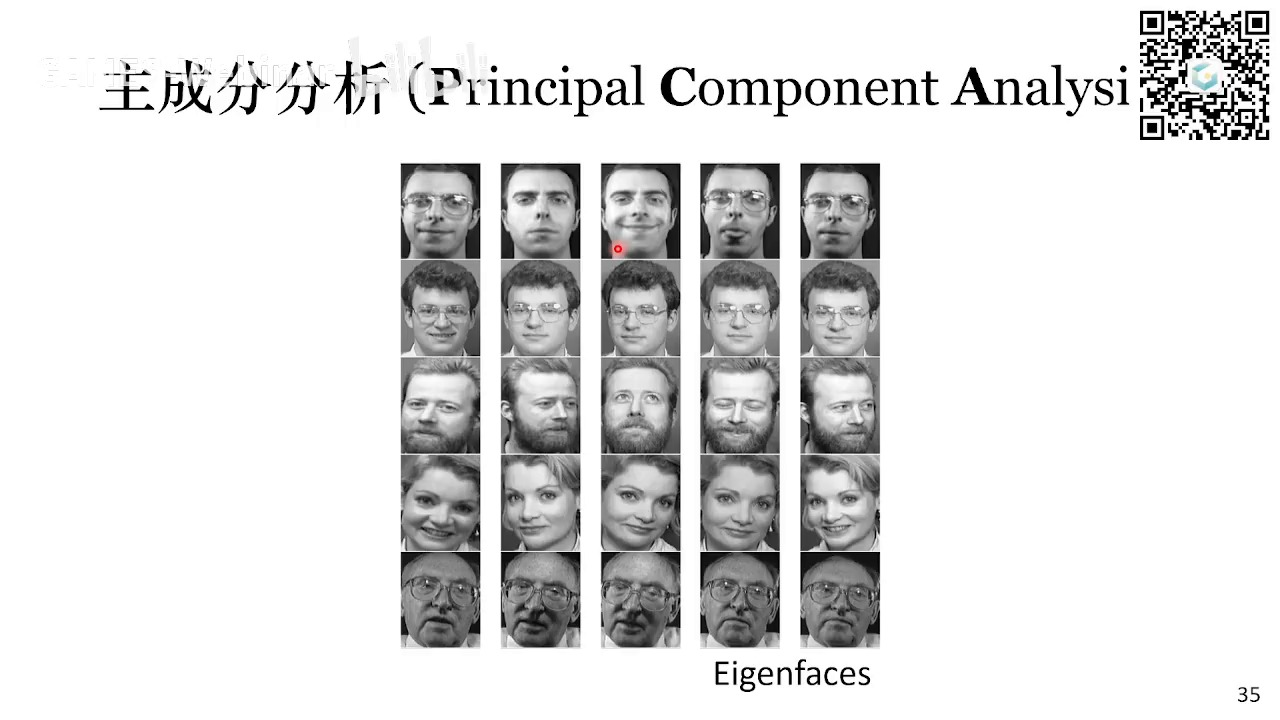
\includegraphics[width=0.92\textwidth]{figures/fig_32_pca_eigenfaces.jpg}
\caption{主成分分析的经典例子 Eigenfaces\vtag}
\end{figure}
\srcnote{01:27:45--01:28:00}
\end{minipage}


\noindent\begin{minipage}{\textwidth}
\begin{figure}[H]
\centering
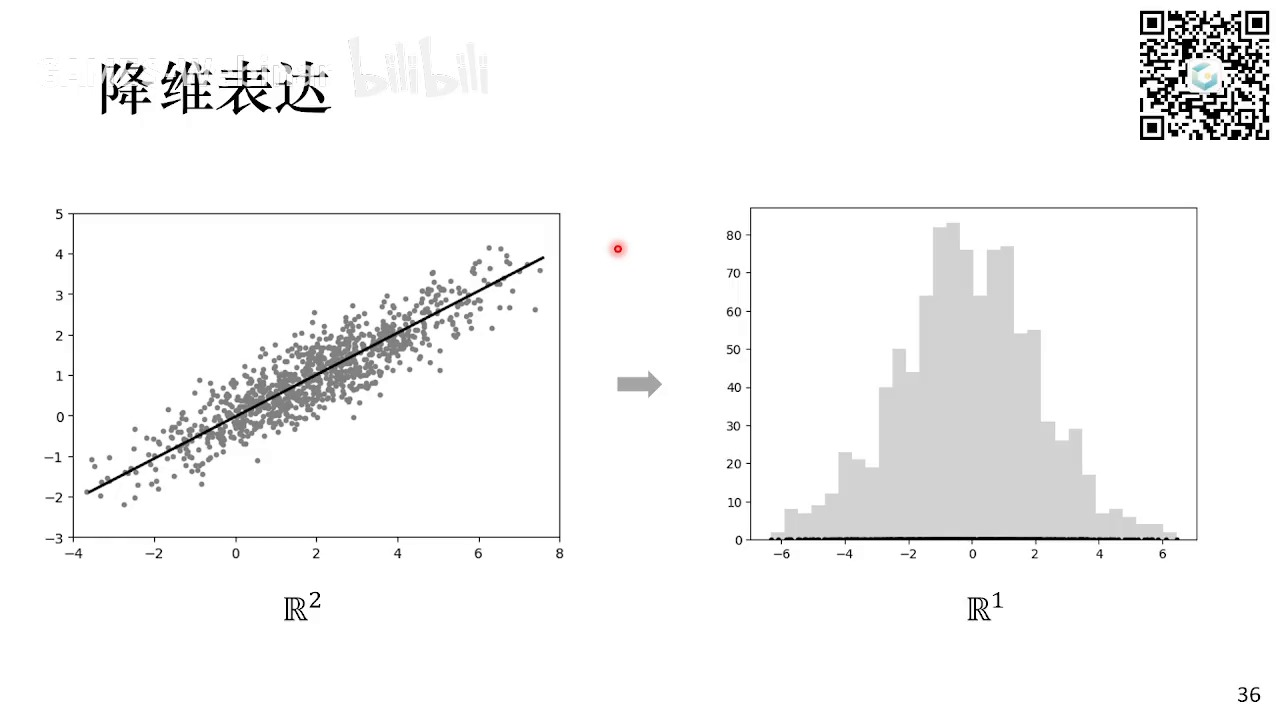
\includegraphics[width=0.92\textwidth]{figures/fig_33_dim_reduce.jpg}
\caption{降维表达：把 $\mathbb R^2$ 中的数据投影到 $\mathbb R^1$\vtag}
\end{figure}
\srcnote{01:29:00--01:29:15}
\end{minipage}


\subsection{零阶近似：只有一个点}

数据集为 $\mathbf x_0,\dots,\mathbf x_{k-1}\in\mathbb R^n$。如果只能用一个点 $\mathbf m$ 代表整个数据集，应该让它到所有点的距离平方和最小：
\[
\mathbf m=\operatorname*{argmin}_{\mathbf x}\sum_{i=0}^{k-1}\|\mathbf x_i-\mathbf x\|^2
\;\Longrightarrow\;
\mathbf m=\frac1k\sum_{i=0}^{k-1}\mathbf x_i ,
\]
即数据的均值。课件把分母写成了 $n$，按这里的记号应为数据点个数 $k$。

\begin{warningbox}{PCA 之前一定要中心化}
零阶近似的结论有一个直接的实践含义：后面所有的主方向都是围绕均值 $\mathbf m$ 定义的，方差矩阵里用的是 $\mathbf x_i-\mathbf m$。如果忘了先减去均值，直接对原始数据求 $\sum\mathbf x_i\mathbf x_i^{\mathsf T}$ 的特征向量，第一个“主成分”往往只是指向数据均值的方向，而不是数据真正散开的方向。用 SVD 实现 PCA 时同样要先对数据矩阵按列减去均值。
\end{warningbox}

\noindent\begin{minipage}{\textwidth}
\begin{figure}[H]
\centering
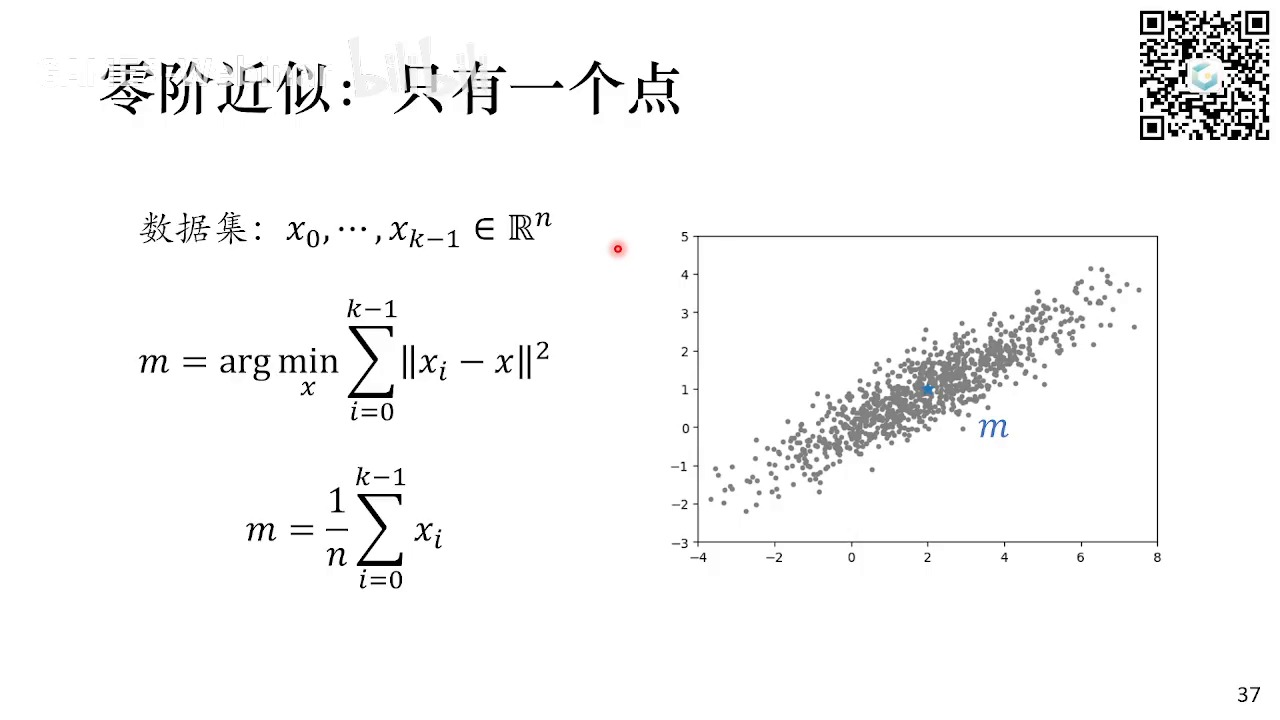
\includegraphics[width=0.92\textwidth]{figures/fig_34_zeroth.jpg}
\caption{零阶近似：用均值点代表数据集\vtag}
\end{figure}
\srcnote{01:29:15--01:29:30}
\end{minipage}


\subsection{一阶近似：主方向}

任意单位方向 $\mathbf v\in\mathbb R^n$，$\|\mathbf v\|=1$，定义一条过均值的直线 $\mathbf x=\mathbf m+t\mathbf v$。把数据点投影到直线上，投影长度为 $x'_i=(\mathbf x_i-\mathbf m)\cdot\mathbf v$；数据点到直线的垂直距离满足勾股定理
\[
d_i^2=\|\mathbf x_i-\mathbf m\|^2-x_i'^2 .
\]
$\|\mathbf x_i-\mathbf m\|$ 与方向无关，所以最小化距离等价于最大化投影：
\[
\operatorname*{argmin}_{\mathbf v}\sum_i d_i^2=\operatorname*{argmax}_{\mathbf v}\sum_i x_i'^2=\operatorname*{argmax}_{\mathbf v}\ \mathbf v^{\mathsf T}\Big(\sum_i(\mathbf x_i-\mathbf m)(\mathbf x_i-\mathbf m)^{\mathsf T}\Big)\mathbf v .
\]
括号里的矩阵记为 $\mathrm S$，称为方差（协方差）矩阵。直观上，好的方向让投影后的点分布得尽量开，坏的方向让它们挤在一起。

\noindent\begin{minipage}{\textwidth}
\begin{figure}[H]
\centering
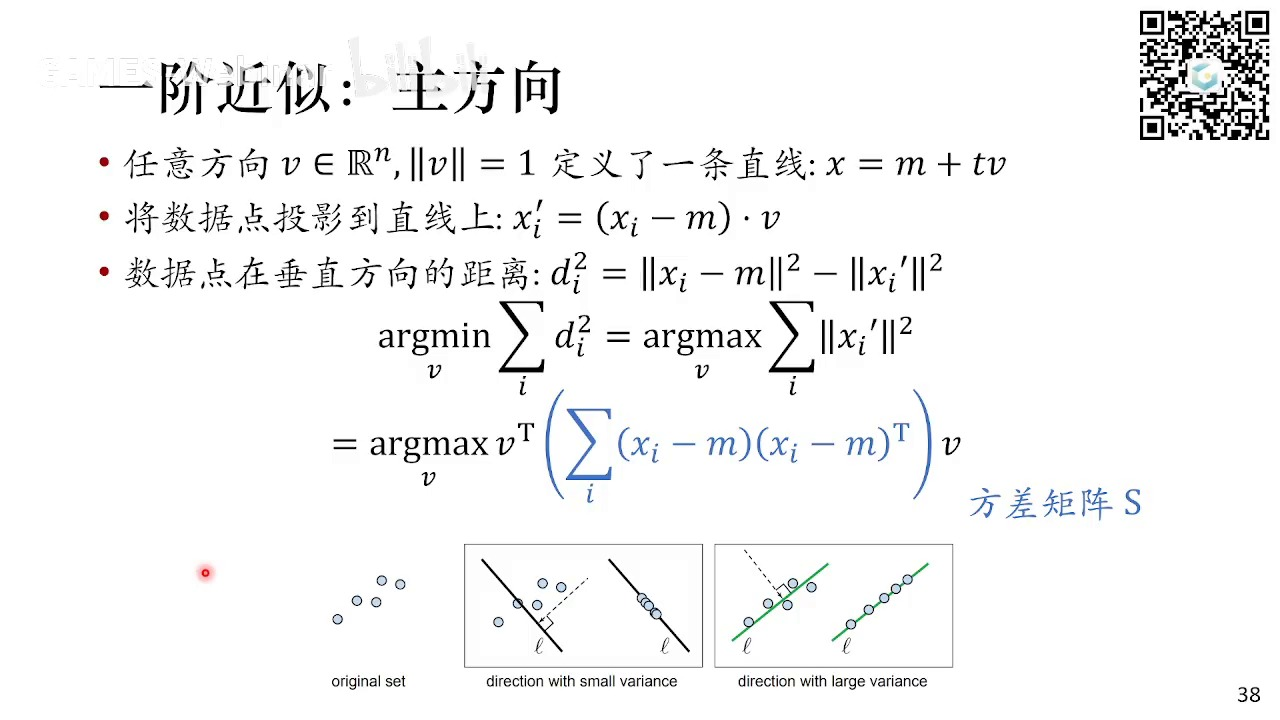
\includegraphics[width=0.92\textwidth]{figures/fig_35_first_order.jpg}
\caption{一阶近似：最小化到直线的距离等价于最大化投影方差\vtag}
\end{figure}
\srcnote{01:32:00--01:32:15}
\end{minipage}


$\mathrm S\in\mathbb R^{n\times n}$ 是半正定矩阵，可以实数对角化，特征值非负且排序为 $\lambda_0\ge\lambda_1\ge\cdots\ge0$：
\[
\mathbf v^{\mathsf T}\mathrm S\mathbf v=\mathbf v^{\mathsf T}\mathrm Q\Lambda\mathrm Q^{\mathsf T}\mathbf v=(\mathrm Q^{\mathsf T}\mathbf v)^{\mathsf T}\Lambda(\mathrm Q^{\mathsf T}\mathbf v).
\]
$\mathrm Q^{\mathsf T}\mathbf v$ 仍是单位向量，所以这是 $\Lambda$ 对角元的加权平均，最大值为 $\lambda_0$，在 $\mathbf v=\mathbf q_0$，即 $\mathrm Q^{\mathsf T}\mathbf v=(1,0,\dots,0)^{\mathsf T}$ 时取到。所以主方向 $\mathbf p$ 是方差矩阵最大特征值对应的特征向量。

\noindent\begin{minipage}{\textwidth}
\begin{figure}[H]
\centering
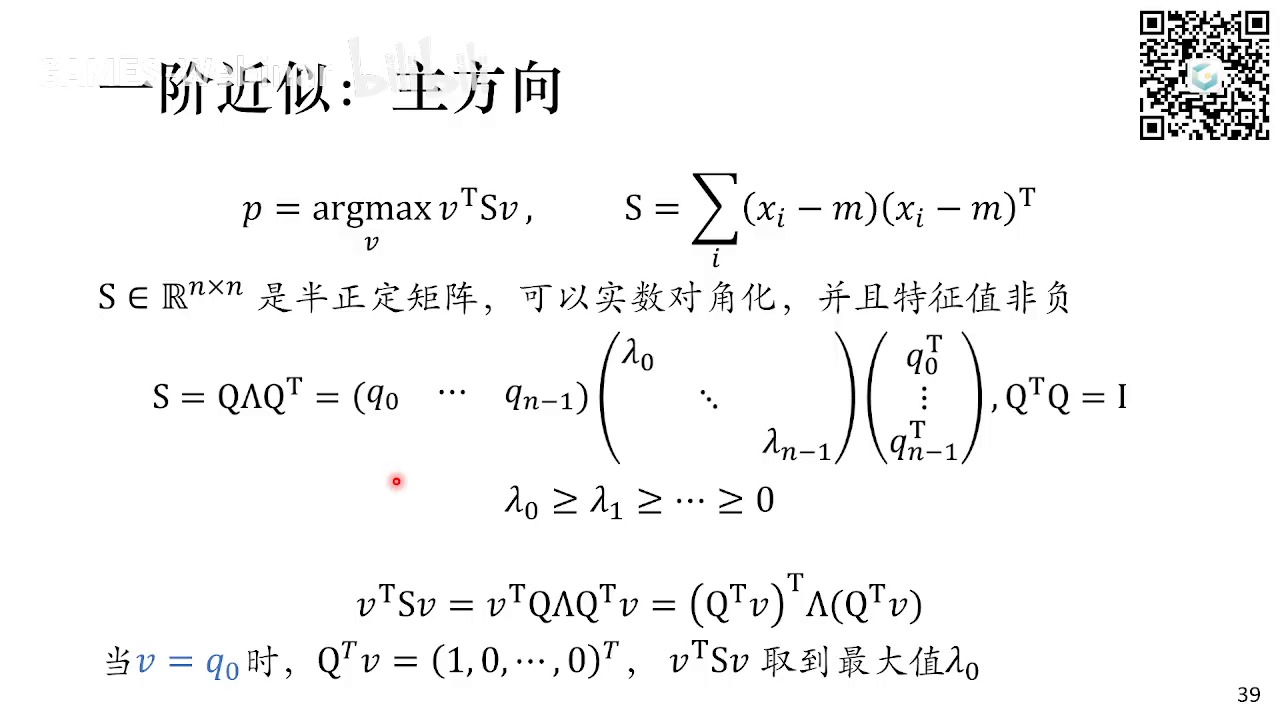
\includegraphics[width=0.92\textwidth]{figures/fig_36_first_order_eig.jpg}
\caption{主方向是方差矩阵最大特征值对应的特征向量\vtag}
\end{figure}
\srcnote{01:35:15--01:35:30}
\end{minipage}


\subsection{继续下去}

找到第一个主方向 $\mathbf p$ 后，从数据中减去它方向上的分量：
\[
\mathbf x''_i=\mathbf x_i-\mathbf m-\big((\mathbf x_i-\mathbf m)\cdot\mathbf p\big)\mathbf p ,
\]
再对剩下的分量找主方向：
\[
\operatorname*{argmax}_{\mathbf v}\ \mathbf v^{\mathsf T}\Big(\sum_i\mathbf x''_i\mathbf x''^{\mathsf T}_i\Big)\mathbf v=\operatorname*{argmax}_{\mathbf v}\ \mathbf v^{\mathsf T}(\mathrm S-\lambda_0\mathbf p\mathbf p^{\mathsf T})\mathbf v .
\]
由于 $\mathrm S=\lambda_0\mathbf q_0\mathbf q_0^{\mathsf T}+\lambda_1\mathbf q_1\mathbf q_1^{\mathsf T}+\cdots$，减去第一项后，最大特征值变成 $\lambda_1$，第二个主方向就是 $\mathbf q_1$。讲者建议读者自己把这一步推出来。

\noindent\begin{minipage}{\textwidth}
\begin{figure}[H]
\centering
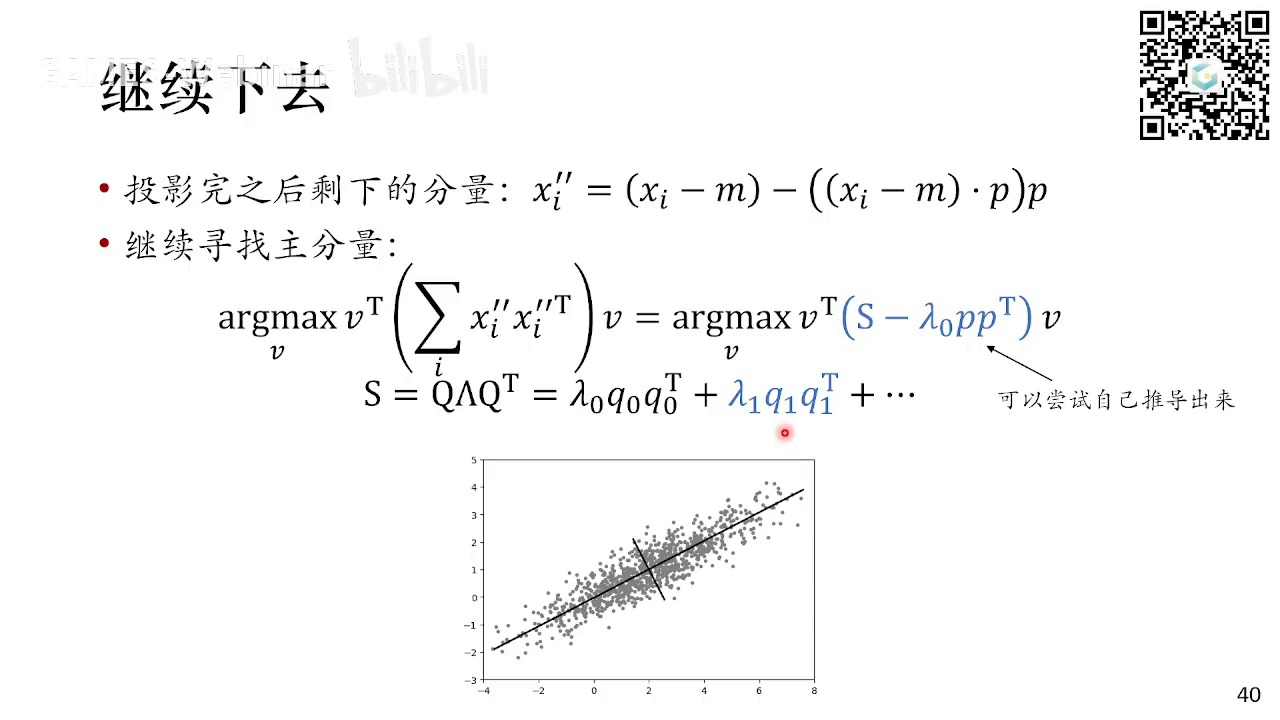
\includegraphics[width=0.92\textwidth]{figures/fig_37_pca_continue.jpg}
\caption{逐次去掉已找到的主方向，依次得到后续主成分\vtag}
\end{figure}
\srcnote{01:37:45--01:38:00}
\end{minipage}


\begin{importantbox}{PCA 的结论}
由 $k$ 个 $n$ 维数据点 $\mathbf x_0,\dots,\mathbf x_{k-1}$ 组成的数据集，前 $m$ 个主成分是方差矩阵 $\mathrm S=\sum_i(\mathbf x_i-\bar{\mathbf x})(\mathbf x_i-\bar{\mathbf x})^{\mathsf T}$ 的前 $m$ 个特征向量 $\mathbf q_0,\dots,\mathbf q_{m-1}$（课件中均值也记作 $\mathbf m$，这里写作 $\bar{\mathbf x}$ 以免与维数 $m$ 混淆）。这些向量相互正交，张成一个 $m$ 维子空间；把数据投影到这个子空间，就得到数据集的低维表达。实际计算时，也可以直接对中心化后的数据矩阵做 SVD，其右奇异向量就是主成分。
\end{importantbox}

\noindent\begin{minipage}{\textwidth}
\begin{figure}[H]
\centering
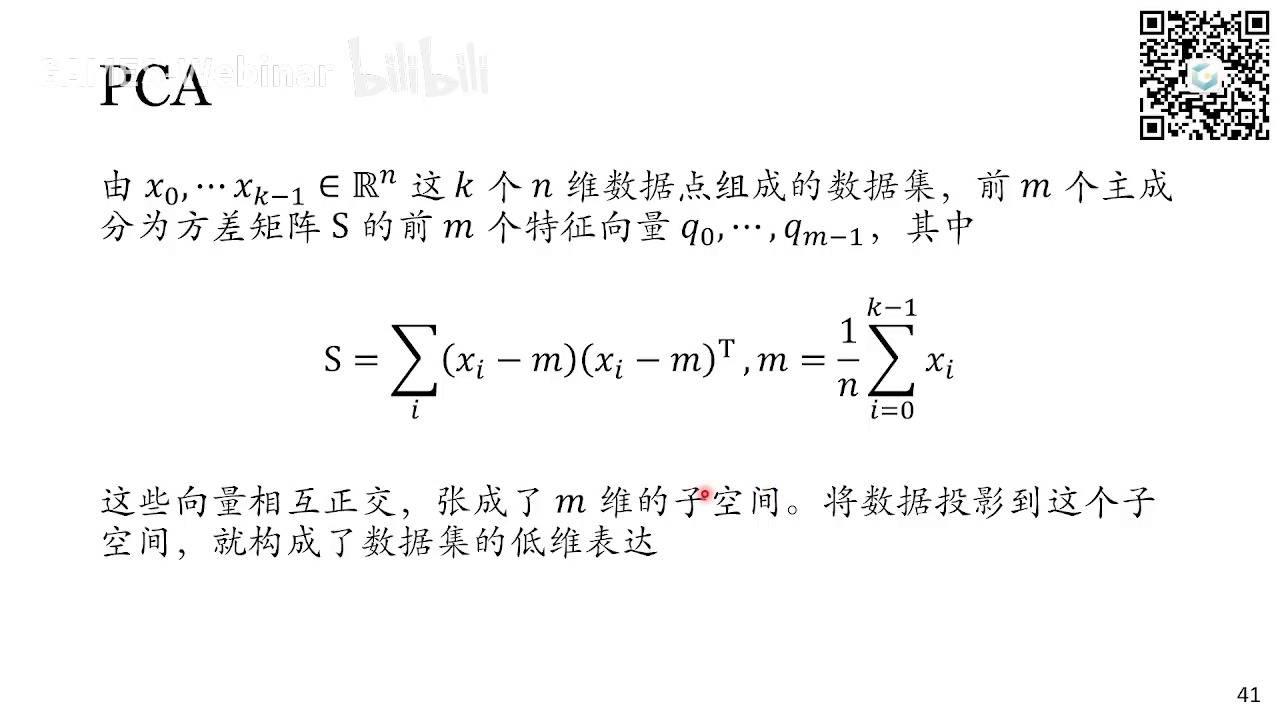
\includegraphics[width=0.92\textwidth]{figures/fig_38_pca_summary.jpg}
\caption{PCA 的结论：前 $m$ 个主成分即方差矩阵的前 $m$ 个特征向量\vtag}
\end{figure}
\srcnote{01:38:45--01:39:00}
\end{minipage}


\begin{knowledgebox}{PCA 与 SVD 的关系}
讲义作者补充：把中心化后的数据按行排成矩阵 $\mathrm X\in\mathbb R^{k\times n}$，则方差矩阵 $\mathrm S=\mathrm X^{\mathsf T}\mathrm X$。若 $\mathrm X=\mathrm U\Sigma\mathrm V^{\mathsf T}$，则 $\mathrm S=\mathrm V\Sigma^{\mathsf T}\Sigma\mathrm V^{\mathsf T}$，即 $\mathrm X$ 的右奇异向量就是主成分，奇异值的平方就是各主成分方向上的方差。这正是本讲把 SVD 和 PCA 放在一起讲的原因：前半讲的低秩近似（图像压缩）和后半讲的降维（PCA）其实是同一件事在不同数据上的体现。数值上，直接对 $\mathrm X$ 做 SVD 也比先算 $\mathrm X^{\mathsf T}\mathrm X$ 再求特征值更稳定。
\end{knowledgebox}

\section{PCA 的应用与局限}

\subsection{点云法向}

点云本身没有法向信息。取表面上一点和它的邻域点做 PCA，前两个主方向张成切平面，方差最小的第三个主方向就是法向。讲者的解释是：把一点周围的邻居点拿出来作为一个三维数据集，求它的第一和第二主分量；对于足够小的邻域，表面近似是平的，点主要沿着表面散开，所以这两个主分量对应的是该点处的切平面，与它们都垂直的方向就是法向。需要注意，PCA 只能给出无符号的方向，法向朝内还是朝外，需要别的算法来确定。

\noindent\begin{minipage}{\textwidth}
\begin{figure}[H]
\centering
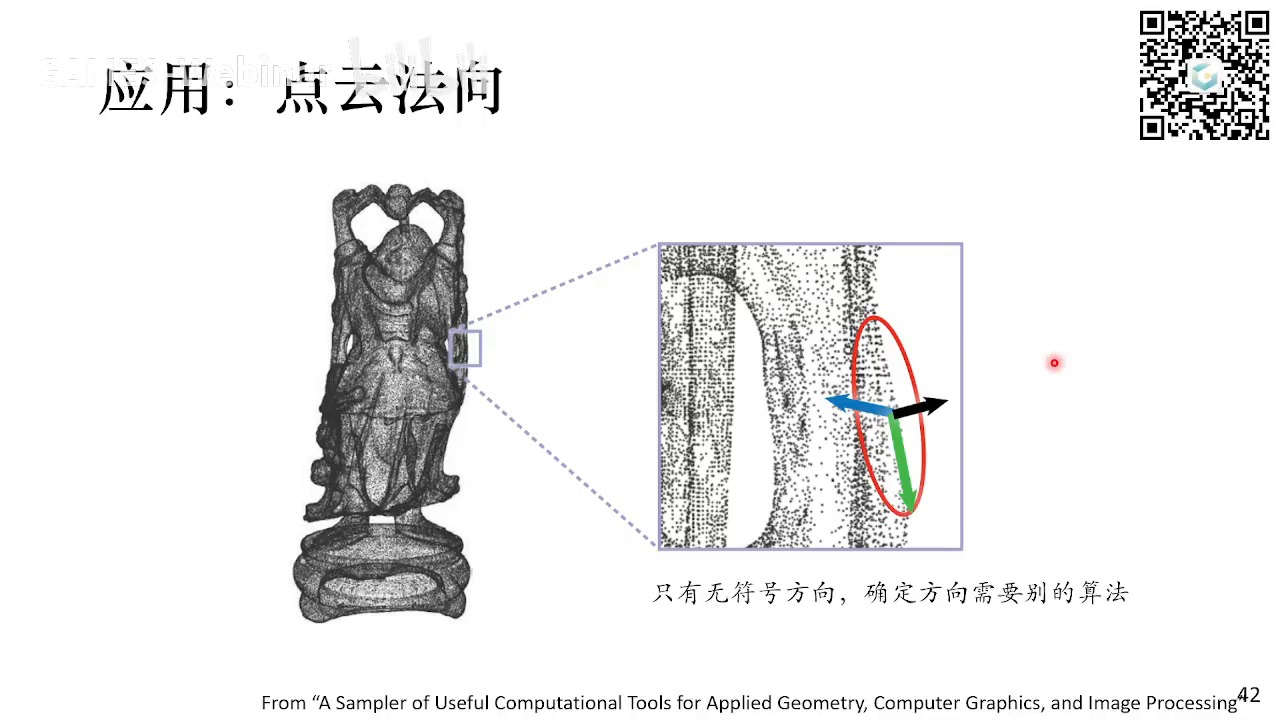
\includegraphics[width=0.92\textwidth]{figures/fig_39_normals.jpg}
\caption{点云法向：邻域点 PCA 的最小主方向；只能给出无符号方向\vtag}
\end{figure}
\srcnote{01:40:30--01:40:45}
\end{minipage}


\subsection{Eigenfaces}

课件中的例子用了 400 张 $112\times92$ 的人脸图片。每张图片是一个数据点，维数是 $112\times92$，空间非常大。对这 400 个数据点做 PCA，提取前 40 个主分量，画出来就是 40 张 Eigenfaces，单独看看不出是什么。每张人脸都可以近似表示为这 40 个主分量的线性组合，于是 400 张图片被压缩成 400 个 40 维的权重向量。用权重重建出的人脸大多和原图很像，但也有一些明显的瑕疵。整体来说，重建结果和原数据集的分布是很接近的，这就是原数据集的降维表达：每个数据点原来有 $112\times92$ 维，现在只需要 40 维的权重，因为它被投影到了 40 个主成分张成的子空间里。

\noindent\begin{minipage}{\textwidth}
\begin{figure}[H]
\centering
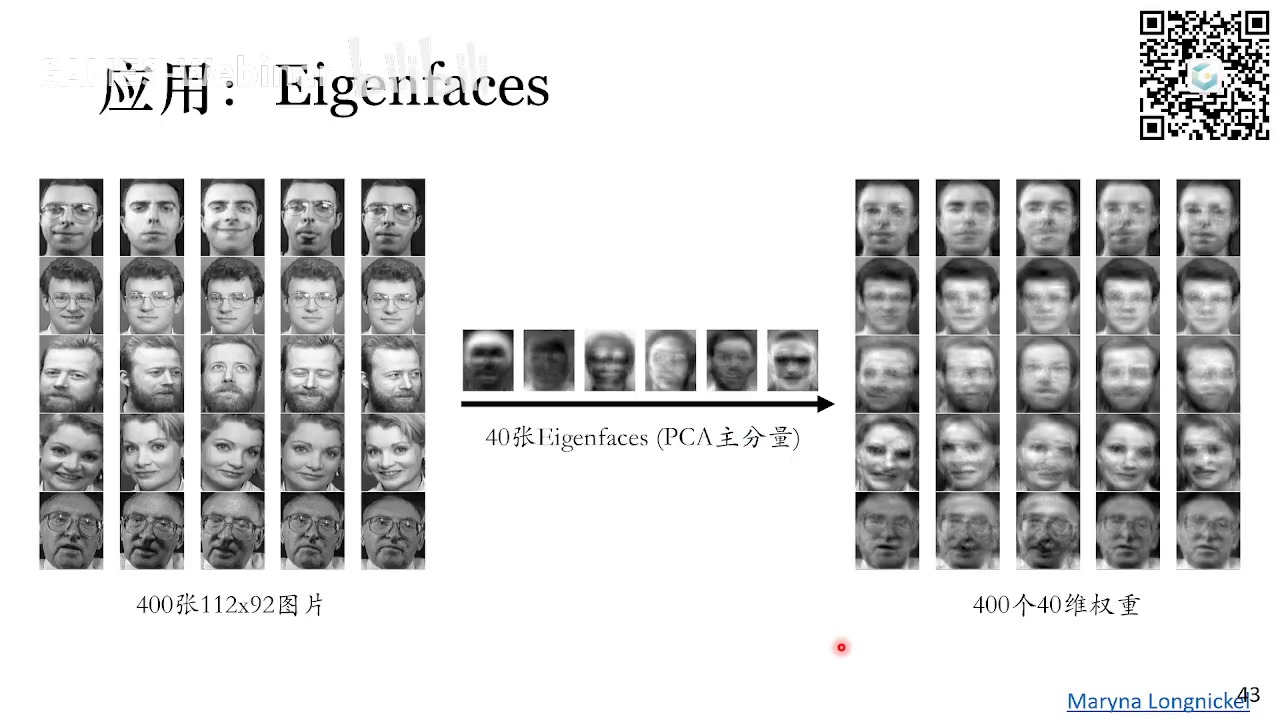
\includegraphics[width=0.92\textwidth]{figures/fig_40_eigenfaces.jpg}
\caption{Eigenfaces：400 张 $112\times92$ 图片、40 个主分量、400 个 40 维权重\vtag}
\end{figure}
\srcnote{01:42:45--01:43:00}
\end{minipage}


\subsection{模型降阶}

PCA 在物理模拟中的应用是模型降阶（model reduction），也叫本征正交分解（proper orthogonal decomposition, POD）。完整模拟的自由度很多，因为网格有很多节点，开销很大。可以预先跑很多次模拟，把每一帧的状态当成数据点，对它们做 PCA 降维；之后只在少数主成分张成的子空间里模拟，自由度大大减少。由于主成分是原数据集的近似，降阶模拟的结果也会和之前的完整模拟相像。这样就可以用来帮助模拟加速，后续的物理模拟课程里还会看到这类应用。它的前提是：之后要模拟的运动，和预先跑过的那些模拟属于“同一类”，落在相同的低维子空间附近。

\noindent\begin{minipage}{\textwidth}
\begin{figure}[H]
\centering
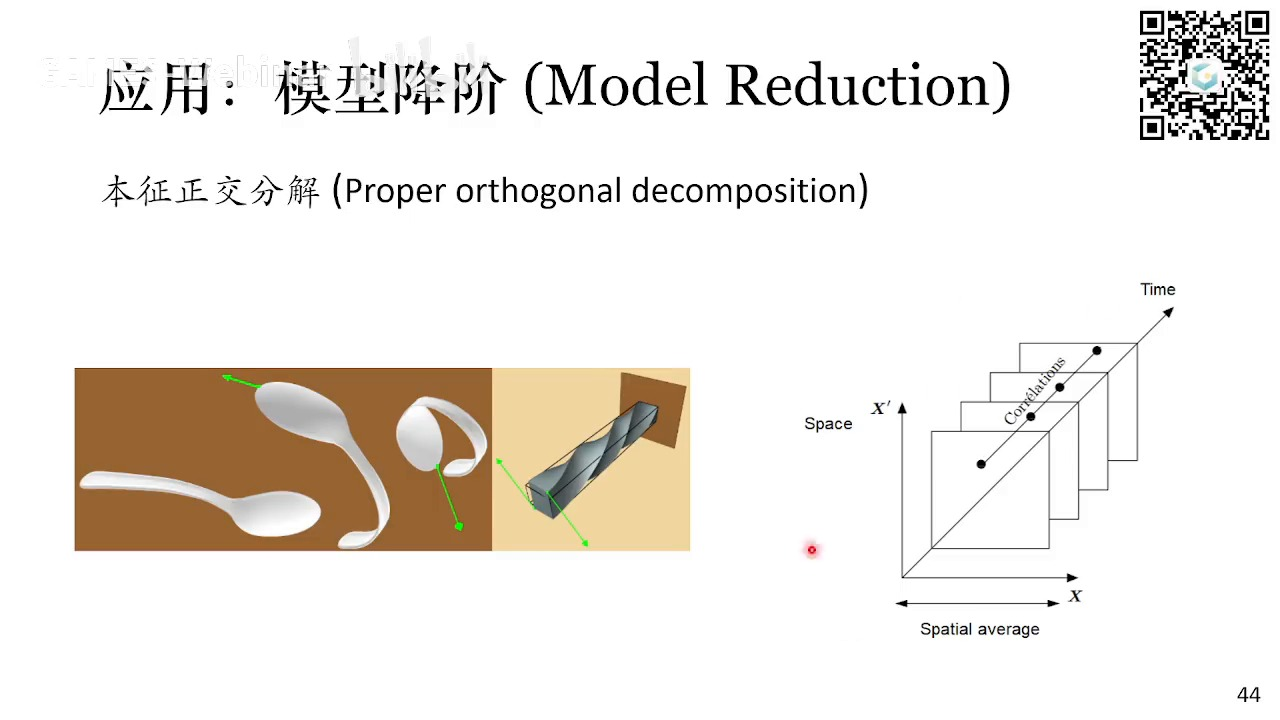
\includegraphics[width=0.92\textwidth]{figures/fig_41_model_reduction.jpg}
\caption{模型降阶：对模拟数据做 PCA，在低维子空间中模拟\vtag}
\end{figure}
\srcnote{01:44:15--01:44:30}
\end{minipage}


\subsection{非线性数据}

PCA 的局限是它只能找线性子空间。例如所有点分布在一个圆圈上，本质上是一维的数据集，但 PCA 只能找到直线方向，无法用一维表达它。更具体地说，对分布在圆上的数据做 PCA，前两个主分量张成的是圆所在的平面，于是只能得到一个二维的近似，无法揭示“其实只有一个角度在变化”这一特征。这时 PCA 也不是不能用，只是效果不好。解决方法之一是 Kernel PCA，先把数据映射到高维特征空间再做 PCA；现在更常用的是编码器—解码器（encoder--decoder）结构的神经网络，直接学习非线性的降维与重建。编码器通过若干神经网络层把高维向量映射到低维的隐空间（latent code），解码器再把隐向量恢复成高维数据；训练的目标是让恢复结果尽量接近输入，这可以看作 PCA“投影—重建”思想的非线性推广。

\noindent\begin{minipage}{\textwidth}
\begin{figure}[H]
\centering
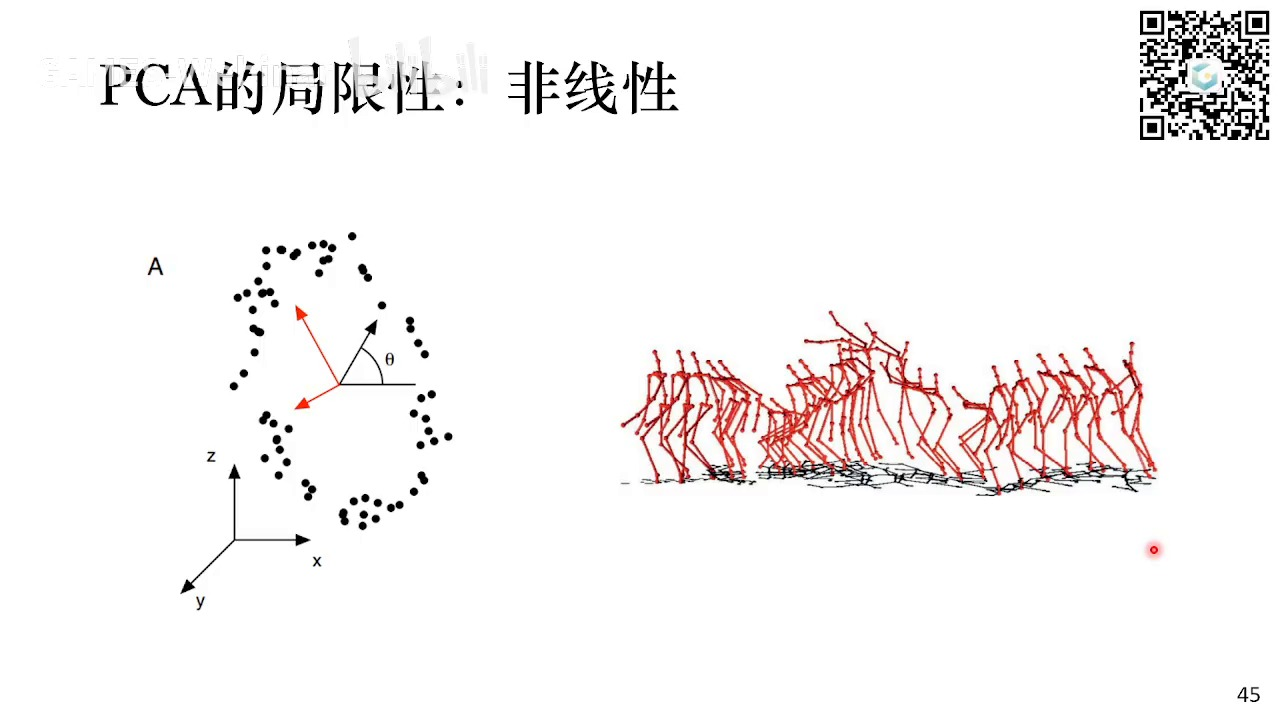
\includegraphics[width=0.92\textwidth]{figures/fig_42_pca_nonlinear.jpg}
\caption{PCA 的局限：非线性分布的数据\vtag}
\end{figure}
\srcnote{01:46:00--01:46:15}
\end{minipage}


\noindent\begin{minipage}{\textwidth}
\begin{figure}[H]
\centering
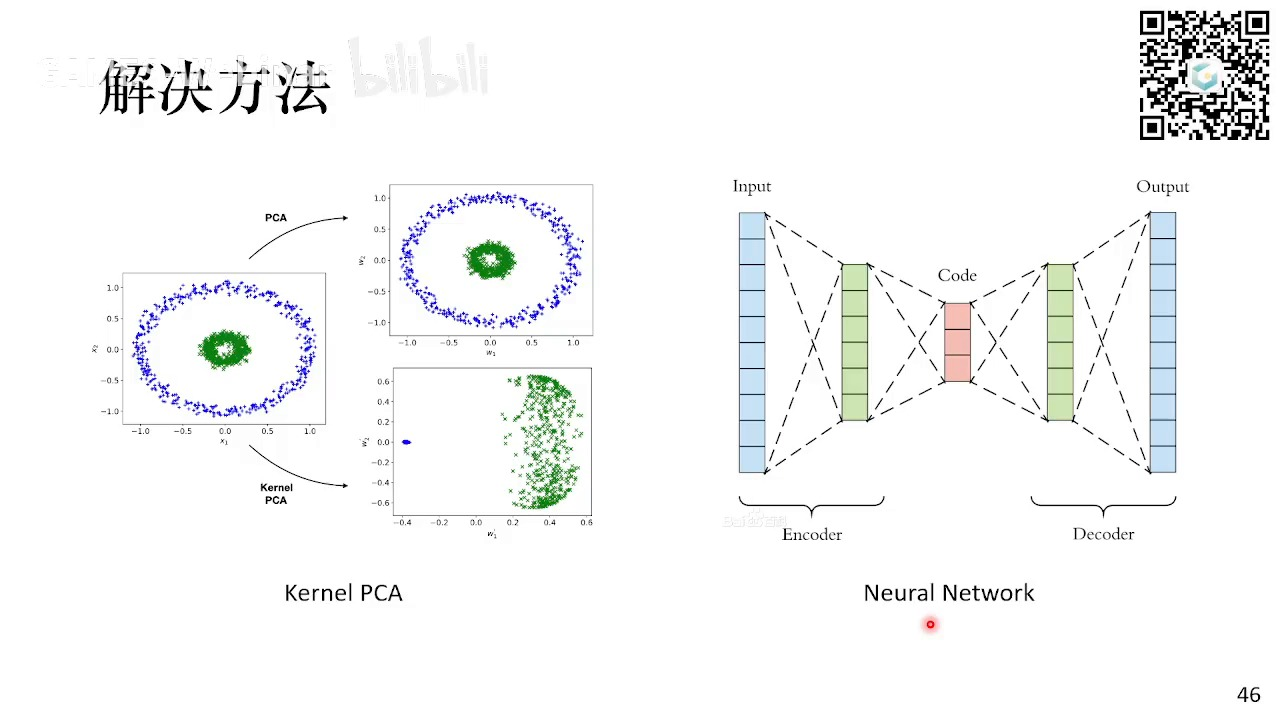
\includegraphics[width=0.92\textwidth]{figures/fig_43_kernel_nn.jpg}
\caption{解决方法：Kernel PCA 与神经网络\vtag}
\end{figure}
\srcnote{01:48:00--01:48:15}
\end{minipage}


\section{参考资料与自测}

讲者列出的参考资料有：Daniel Cohen-Or 的图形学课程（cs.tau.ac.il/\textasciitilde dcor/Graphics），Gilbert Strang 的 MIT 线性代数讲义，Eftychios Sifakis 关于有限元弹性体模拟的讲义，以及 Olga Sorkine-Hornung 关于最优旋转的笔记。

\begin{practicebox}{自测清单}
\begin{itemize}
\item 证明实对称矩阵特征值为实数、不同特征值的特征向量正交。
\item 从 $\mathrm A^{\mathsf T}\mathrm A$ 的特征分解出发写出 SVD，并说明 $\Sigma$ 的形状和非零对角元个数。
\item 分别推导超定方程的左逆、欠定方程的右逆，说明二者何时与伪逆相等。
\item 用 SVD 写出极分解的两种形式，说明两者中的旋转相同、拉伸不同。
\item 写出形状匹配的四步算法，并解释 $\det(\mathrm V\mathrm U^{\mathsf T})=-1$ 时如何修正。
\item 计算保留 $k$ 个奇异值时 $512\times512$ 图像的存储比。
\item 推导 $\delta\Sigma=\operatorname{Diag}(\mathrm U^{\mathsf T}\delta\mathrm F\mathrm V)$。
\item 说明 PCA 的主方向为什么是协方差矩阵最大特征值的特征向量，以及它如何用于点云法向估计。
\end{itemize}
\end{practicebox}

\end{document}
